%%
%DIF LATEXDIFF DIFFERENCE FILE
%DIF DEL ms/LMA_method_old.tex   Wed Apr 13 01:19:52 2022
%DIF ADD ms/LMA_method.tex       Fri May 13 18:54:39 2022
% Copyright (c) 2017 - 2020, Pascal Wagler;
% Copyright (c) 2014 - 2020, John MacFarlane
%
% All rights reserved.
%
% Redistribution and use in source and binary forms, with or without
% modification, are permitted provided that the following conditions
% are met:
%
% - Redistributions of source code must retain the above copyright
% notice, this list of conditions and the following disclaimer.
%
% - Redistributions in binary form must reproduce the above copyright
% notice, this list of conditions and the following disclaimer in the
% documentation and/or other materials provided with the distribution.
%
% - Neither the name of John MacFarlane nor the names of other
% contributors may be used to endorse or promote products derived
% from this software without specific prior written permission.
%
% THIS SOFTWARE IS PROVIDED BY THE COPYRIGHT HOLDERS AND CONTRIBUTORS
% "AS IS" AND ANY EXPRESS OR IMPLIED WARRANTIES, INCLUDING, BUT NOT
% LIMITED TO, THE IMPLIED WARRANTIES OF MERCHANTABILITY AND FITNESS
% FOR A PARTICULAR PURPOSE ARE DISCLAIMED. IN NO EVENT SHALL THE
% COPYRIGHT OWNER OR CONTRIBUTORS BE LIABLE FOR ANY DIRECT, INDIRECT,
% INCIDENTAL, SPECIAL, EXEMPLARY, OR CONSEQUENTIAL DAMAGES (INCLUDING,
% BUT NOT LIMITED TO, PROCUREMENT OF SUBSTITUTE GOODS OR SERVICES;
% LOSS OF USE, DATA, OR PROFITS; OR BUSINESS INTERRUPTION) HOWEVER
% CAUSED AND ON ANY THEORY OF LIABILITY, WHETHER IN CONTRACT, STRICT
% LIABILITY, OR TORT (INCLUDING NEGLIGENCE OR OTHERWISE) ARISING IN
% ANY WAY OUT OF THE USE OF THIS SOFTWARE, EVEN IF ADVISED OF THE
% POSSIBILITY OF SUCH DAMAGE.
%%

%%
% This is the Eisvogel pandoc LaTeX template.
%
% For usage information and examples visit the official GitHub page:
% https://github.com/Wandmalfarbe/pandoc-latex-template
%%

\DeclareUnicodeCharacter{2212}{-}

% Options for packages loaded elsewhere
\PassOptionsToPackage{unicode}{hyperref}
\PassOptionsToPackage{hyphens}{url}
\PassOptionsToPackage{dvipsnames,svgnames*,x11names*,table}{xcolor}
%
\documentclass[
  12pt,
  a4paper,
,tablecaptionabove
]{scrartcl}
\usepackage{lmodern}
\usepackage{setspace}
\setstretch{1.2}
\usepackage{amssymb,amsmath}
\usepackage{ifxetex,ifluatex}
\ifnum 0\ifxetex 1\fi\ifluatex 1\fi=0 % if pdftex
  \usepackage[T1]{fontenc}
  \usepackage[utf8]{inputenc}
  \usepackage{textcomp} % provide euro and other symbols
\else % if luatex or xetex
  \usepackage{unicode-math}
  \defaultfontfeatures{Scale=MatchLowercase}
  \defaultfontfeatures[\rmfamily]{Ligatures=TeX,Scale=1}
\fi
% Use upquote if available, for straight quotes in verbatim environments
\IfFileExists{upquote.sty}{\usepackage{upquote}}{}
\IfFileExists{microtype.sty}{% use microtype if available
  \usepackage[]{microtype}
  \UseMicrotypeSet[protrusion]{basicmath} % disable protrusion for tt fonts
}{}
\makeatletter
\@ifundefined{KOMAClassName}{% if non-KOMA class
  \IfFileExists{parskip.sty}{%
    \usepackage{parskip}
  }{% else
    \setlength{\parindent}{0pt}
    \setlength{\parskip}{6pt plus 2pt minus 1pt}}
}{% if KOMA class
  \KOMAoptions{parskip=half}}
\makeatother
\usepackage{xcolor}
\definecolor{default-linkcolor}{HTML}{A50000}
\definecolor{default-filecolor}{HTML}{A50000}
\definecolor{default-citecolor}{HTML}{4077C0}
\definecolor{default-urlcolor}{HTML}{4077C0}
\IfFileExists{xurl.sty}{\usepackage{xurl}}{} % add URL line breaks if available
\IfFileExists{bookmark.sty}{\usepackage{bookmark}}{\usepackage{hyperref}}
\hypersetup{
  hidelinks,
  breaklinks=true,
  pdfcreator={LaTeX via pandoc with the Eisvogel template}}
\urlstyle{same} % disable monospaced font for URLs
\usepackage[margin=1in]{geometry}
\usepackage{longtable,booktabs}
% Correct order of tables after \paragraph or \subparagraph
\usepackage{etoolbox}
\makeatletter
\patchcmd\longtable{\par}{\if@noskipsec\mbox{}\fi\par}{}{}
\makeatother
% Allow footnotes in longtable head/foot
\IfFileExists{footnotehyper.sty}{\usepackage{footnotehyper}}{\usepackage{footnote}}
\makesavenoteenv{longtable}
% add backlinks to footnote references, cf. https://tex.stackexchange.com/questions/302266/make-footnote-clickable-both-ways
\usepackage{footnotebackref}
\usepackage{graphicx}
\makeatletter
\def\maxwidth{\ifdim\Gin@nat@width>\linewidth\linewidth\else\Gin@nat@width\fi}
\def\maxheight{\ifdim\Gin@nat@height>\textheight\textheight\else\Gin@nat@height\fi}
\makeatother
% Scale images if necessary, so that they will not overflow the page
% margins by default, and it is still possible to overwrite the defaults
% using explicit options in \includegraphics[width, height, ...]{}
\setkeys{Gin}{width=\maxwidth,height=\maxheight,keepaspectratio}
\setlength{\emergencystretch}{3em}  % prevent overfull lines
\providecommand{\tightlist}{%
  \setlength{\itemsep}{0pt}\setlength{\parskip}{0pt}}
\setcounter{secnumdepth}{-\maxdimen} % remove section numbering

% Make use of float-package and set default placement for figures to H.
% The option H means 'PUT IT HERE' (as  opposed to the standard h option which means 'You may put it here if you like').
\usepackage{float}
\floatplacement{figure}{H}

\usepackage{booktabs}
\usepackage{longtable}
\usepackage{array}
\usepackage{multirow}
\usepackage{wrapfig}
\usepackage{float}
\usepackage{colortbl}
\usepackage{pdflscape}
\usepackage{tabu}
\usepackage{threeparttable}
\usepackage{threeparttablex}
\usepackage[normalem]{ulem}
\usepackage{makecell}
\usepackage{xcolor}
\usepackage{lineno}
\linenumbers

\newlength{\cslhangindent}
\setlength{\cslhangindent}{1.5em}
\newlength{\csllabelwidth}
\setlength{\csllabelwidth}{3em}
\newenvironment{CSLReferences}[2] % #1 hanging-ident, #2 entry spacing
 {% don't indent paragraphs
  \setlength{\parindent}{0pt}
  % turn on hanging indent if param 1 is 1
  \ifodd #1 \everypar{\setlength{\hangindent}{\cslhangindent}}\ignorespaces\fi
  % set entry spacing
  \ifnum #2 > 0
  \setlength{\parskip}{#2\baselineskip}
  \fi
 }%
 {}
\usepackage{calc}
\newcommand{\CSLBlock}[1]{#1\hfill\break}
\newcommand{\CSLLeftMargin}[1]{\parbox[t]{\csllabelwidth}{#1}}
\newcommand{\CSLRightInline}[1]{\parbox[t]{\linewidth - \csllabelwidth}{#1}\break}
\newcommand{\CSLIndent}[1]{\hspace{\cslhangindent}#1}

\date{}


%%
%% added
%%

%
% language specification
%
% If no language is specified, use English as the default main document language.
%

\ifnum 0\ifxetex 1\fi\ifluatex 1\fi=0 % if pdftex
  \usepackage[shorthands=off,main=english]{babel}
\else
    % Workaround for bug in Polyglossia that breaks `\familydefault` when `\setmainlanguage` is used.
  % See https://github.com/Wandmalfarbe/pandoc-latex-template/issues/8
  % See https://github.com/reutenauer/polyglossia/issues/186
  % See https://github.com/reutenauer/polyglossia/issues/127
  \renewcommand*\familydefault{\sfdefault}
    % load polyglossia as late as possible as it *could* call bidi if RTL lang (e.g. Hebrew or Arabic)
  \usepackage{polyglossia}
  \setmainlanguage[]{english}
\fi



%
% for the background color of the title page
%

%
% break urls
%
\PassOptionsToPackage{hyphens}{url}

%
% When using babel or polyglossia with biblatex, loading csquotes is recommended
% to ensure that quoted texts are typeset according to the rules of your main language.
%
\usepackage{csquotes}

%
% captions
%
%\definecolor{caption-color}{HTML}{777777}
\definecolor{caption-color}{HTML}{37474F}
%\usepackage[font={stretch=1.2}, textfont={color=caption-color}, position=top, skip=4mm, labelfont=bf, singlelinecheck=false, justification=raggedright]{caption}
\usepackage[font={stretch=1}, textfont={color=caption-color}, position=top, skip=2mm, labelfont=bf, singlelinecheck=false, justification=raggedright]{caption}
\setcapindent{0em}

%
% blockquote
%
\definecolor{blockquote-border}{RGB}{221,221,221}
\definecolor{blockquote-text}{RGB}{119,119,119}
\usepackage{mdframed}
\newmdenv[rightline=false,bottomline=false,topline=false,linewidth=3pt,linecolor=blockquote-border,skipabove=\parskip]{customblockquote}
\renewenvironment{quote}{\begin{customblockquote}\list{}{\rightmargin=0em\leftmargin=0em}%
\item\relax\color{blockquote-text}\ignorespaces}{\unskip\unskip\endlist\end{customblockquote}}

%
% Source Sans Pro as the de­fault font fam­ily
% Source Code Pro for monospace text
%
% 'default' option sets the default
% font family to Source Sans Pro, not \sfdefault.
%
\ifnum 0\ifxetex 1\fi\ifluatex 1\fi=0 % if pdftex
    \usepackage[default]{sourcesanspro}
  \usepackage{sourcecodepro}
  %\usepackage{}
  \else % if not pdftex
    \usepackage[default]{sourcesanspro}
  \usepackage{sourcecodepro}
  %\usepackage{}

  % XeLaTeX specific adjustments for straight quotes: https://tex.stackexchange.com/a/354887
  % This issue is already fixed (see https://github.com/silkeh/latex-sourcecodepro/pull/5) but the
  % fix is still unreleased.
  % TODO: Remove this workaround when the new version of sourcecodepro is released on CTAN.
  \ifxetex
    \makeatletter
    \defaultfontfeatures[\ttfamily]
      { Numbers   = \sourcecodepro@figurestyle,
        Scale     = \SourceCodePro@scale,
        Extension = .otf }
    \setmonofont
      [ UprightFont    = *-\sourcecodepro@regstyle,
        ItalicFont     = *-\sourcecodepro@regstyle It,
        BoldFont       = *-\sourcecodepro@boldstyle,
        BoldItalicFont = *-\sourcecodepro@boldstyle It ]
      {SourceCodePro}
    \makeatother
  \fi
  \fi

%
% heading color
%
\definecolor{heading-color}{RGB}{40,40,40}
\addtokomafont{section}{\color{heading-color}}
% When using the classes report, scrreprt, book,
% scrbook or memoir, uncomment the following line.
%\addtokomafont{chapter}{\color{heading-color}}

%
% variables for title and author
%
\usepackage{titling}
\title{}
\author{}

%
% tables
%

\definecolor{table-row-color}{HTML}{F5F5F5}
\definecolor{table-rule-color}{HTML}{999999}

%\arrayrulecolor{black!40}
\arrayrulecolor{table-rule-color}     % color of \toprule, \midrule, \bottomrule
\setlength\heavyrulewidth{0.3ex}      % thickness of \toprule, \bottomrule
\renewcommand{\arraystretch}{1.3}     % spacing (padding)


%
% remove paragraph indention
%
\setlength{\parindent}{0pt}
\setlength{\parskip}{6pt plus 2pt minus 1pt}
\setlength{\emergencystretch}{3em}  % prevent overfull lines

%
%
% Listings
%
%


%
% header and footer
%
\usepackage{fancyhdr}

\fancypagestyle{eisvogel-header-footer}{
  \fancyhead{}
  \fancyfoot{}
  \lhead[]{}
  \chead[]{}
  \rhead[]{}
  %\lfoot[\thepage]{}
  \cfoot[]{}
  \cfoot[]{\thepage}
  \renewcommand{\headrulewidth}{0.0pt}
 % \renewcommand{\footrulewidth}{0.0pt}
 % \renewcommand{\headrulewidth}{0.4pt}
 % \renewcommand{\footrulewidth}{0.4pt}
}
\pagestyle{eisvogel-header-footer}

%%
%% end added
%%
%DIF PREAMBLE EXTENSION ADDED BY LATEXDIFF
%DIF UNDERLINE PREAMBLE %DIF PREAMBLE
\RequirePackage[normalem]{ulem} %DIF PREAMBLE
\RequirePackage{color}\definecolor{RED}{rgb}{1,0,0}\definecolor{BLUE}{rgb}{0,0,1} %DIF PREAMBLE
\providecommand{\DIFaddtex}[1]{{\protect\color{blue}\uwave{#1}}} %DIF PREAMBLE
\providecommand{\DIFdeltex}[1]{{\protect\color{red}\sout{#1}}}                      %DIF PREAMBLE
%DIF SAFE PREAMBLE %DIF PREAMBLE
\providecommand{\DIFaddbegin}{} %DIF PREAMBLE
\providecommand{\DIFaddend}{} %DIF PREAMBLE
\providecommand{\DIFdelbegin}{} %DIF PREAMBLE
\providecommand{\DIFdelend}{} %DIF PREAMBLE
\providecommand{\DIFmodbegin}{} %DIF PREAMBLE
\providecommand{\DIFmodend}{} %DIF PREAMBLE
%DIF FLOATSAFE PREAMBLE %DIF PREAMBLE
\providecommand{\DIFaddFL}[1]{\DIFadd{#1}} %DIF PREAMBLE
\providecommand{\DIFdelFL}[1]{\DIFdel{#1}} %DIF PREAMBLE
\providecommand{\DIFaddbeginFL}{} %DIF PREAMBLE
\providecommand{\DIFaddendFL}{} %DIF PREAMBLE
\providecommand{\DIFdelbeginFL}{} %DIF PREAMBLE
\providecommand{\DIFdelendFL}{} %DIF PREAMBLE
%DIF HYPERREF PREAMBLE %DIF PREAMBLE
\providecommand{\DIFadd}[1]{\texorpdfstring{\DIFaddtex{#1}}{#1}} %DIF PREAMBLE
\providecommand{\DIFdel}[1]{\texorpdfstring{\DIFdeltex{#1}}{}} %DIF PREAMBLE
\newcommand{\DIFscaledelfig}{0.5}
%DIF HIGHLIGHTGRAPHICS PREAMBLE %DIF PREAMBLE
\RequirePackage{settobox} %DIF PREAMBLE
\RequirePackage{letltxmacro} %DIF PREAMBLE
\newsavebox{\DIFdelgraphicsbox} %DIF PREAMBLE
\newlength{\DIFdelgraphicswidth} %DIF PREAMBLE
\newlength{\DIFdelgraphicsheight} %DIF PREAMBLE
% store original definition of \includegraphics %DIF PREAMBLE
\LetLtxMacro{\DIFOincludegraphics}{\includegraphics} %DIF PREAMBLE
\newcommand{\DIFaddincludegraphics}[2][]{{\color{blue}\fbox{\DIFOincludegraphics[#1]{#2}}}} %DIF PREAMBLE
\newcommand{\DIFdelincludegraphics}[2][]{% %DIF PREAMBLE
\sbox{\DIFdelgraphicsbox}{\DIFOincludegraphics[#1]{#2}}% %DIF PREAMBLE
\settoboxwidth{\DIFdelgraphicswidth}{\DIFdelgraphicsbox} %DIF PREAMBLE
\settoboxtotalheight{\DIFdelgraphicsheight}{\DIFdelgraphicsbox} %DIF PREAMBLE
\scalebox{\DIFscaledelfig}{% %DIF PREAMBLE
\parbox[b]{\DIFdelgraphicswidth}{\usebox{\DIFdelgraphicsbox}\\[-\baselineskip] \rule{\DIFdelgraphicswidth}{0em}}\llap{\resizebox{\DIFdelgraphicswidth}{\DIFdelgraphicsheight}{% %DIF PREAMBLE
\setlength{\unitlength}{\DIFdelgraphicswidth}% %DIF PREAMBLE
\begin{picture}(1,1)% %DIF PREAMBLE
\thicklines\linethickness{2pt} %DIF PREAMBLE
{\color[rgb]{1,0,0}\put(0,0){\framebox(1,1){}}}% %DIF PREAMBLE
{\color[rgb]{1,0,0}\put(0,0){\line( 1,1){1}}}% %DIF PREAMBLE
{\color[rgb]{1,0,0}\put(0,1){\line(1,-1){1}}}% %DIF PREAMBLE
\end{picture}% %DIF PREAMBLE
}\hspace*{3pt}}} %DIF PREAMBLE
} %DIF PREAMBLE
\LetLtxMacro{\DIFOaddbegin}{\DIFaddbegin} %DIF PREAMBLE
\LetLtxMacro{\DIFOaddend}{\DIFaddend} %DIF PREAMBLE
\LetLtxMacro{\DIFOdelbegin}{\DIFdelbegin} %DIF PREAMBLE
\LetLtxMacro{\DIFOdelend}{\DIFdelend} %DIF PREAMBLE
\DeclareRobustCommand{\DIFaddbegin}{\DIFOaddbegin \let\includegraphics\DIFaddincludegraphics} %DIF PREAMBLE
\DeclareRobustCommand{\DIFaddend}{\DIFOaddend \let\includegraphics\DIFOincludegraphics} %DIF PREAMBLE
\DeclareRobustCommand{\DIFdelbegin}{\DIFOdelbegin \let\includegraphics\DIFdelincludegraphics} %DIF PREAMBLE
\DeclareRobustCommand{\DIFdelend}{\DIFOaddend \let\includegraphics\DIFOincludegraphics} %DIF PREAMBLE
\LetLtxMacro{\DIFOaddbeginFL}{\DIFaddbeginFL} %DIF PREAMBLE
\LetLtxMacro{\DIFOaddendFL}{\DIFaddendFL} %DIF PREAMBLE
\LetLtxMacro{\DIFOdelbeginFL}{\DIFdelbeginFL} %DIF PREAMBLE
\LetLtxMacro{\DIFOdelendFL}{\DIFdelendFL} %DIF PREAMBLE
\DeclareRobustCommand{\DIFaddbeginFL}{\DIFOaddbeginFL \let\includegraphics\DIFaddincludegraphics} %DIF PREAMBLE
\DeclareRobustCommand{\DIFaddendFL}{\DIFOaddendFL \let\includegraphics\DIFOincludegraphics} %DIF PREAMBLE
\DeclareRobustCommand{\DIFdelbeginFL}{\DIFOdelbeginFL \let\includegraphics\DIFdelincludegraphics} %DIF PREAMBLE
\DeclareRobustCommand{\DIFdelendFL}{\DIFOaddendFL \let\includegraphics\DIFOincludegraphics} %DIF PREAMBLE
%DIF END PREAMBLE EXTENSION ADDED BY LATEXDIFF

\begin{document}

%%
%% begin titlepage
%%

%%
%% end titlepage
%%



Sources and consequences of mismatch between leaf disc and whole-leaf leaf mass per area (LMA)

\[ \]

Phisamai Maenpuen\textsuperscript{1,2,3},
Masatoshi Katabuchi\textsuperscript{1*},
Yusuke Onoda\textsuperscript{4},
Cong Zhou\textsuperscript{1,2},
Jiao-Lin Zhang\textsuperscript{1,3*},
Ya-Jun Chen\textsuperscript{1,3,5}

\[ \]

\textsuperscript{1} CAS Key Laboratory of Tropical Forest Ecology, Xishuangbanna Tropical Botanical Garden, Chinese Academy of Sciences, Menglun, Yunnan 666303, China

\textsuperscript{2} University of Chinese Academy of Sciences, Beijing 100049, China

\textsuperscript{3} Center of Plant Ecology, Core Botanical Gardens, Chinese Academy of Sciences, Yunnan 666303, China

\textsuperscript{4} Graduate School of Agriculture, Kyoto University, Kyoto 606-8502, Japan

\textsuperscript{5} Savanna Ecosystem Research Station, Xishuangbanna Tropical Botanical Garden, Chinese Academy of Sciences, Yuanjiang, Yunnan 6663300, China

\[ \]

\textbf{Corresponding Authors}:

Masatoshi Katabuchi

E-mail: \href{mailto:mattocci27@gmail.com}{\nolinkurl{mattocci27@gmail.com}}

Jiao-Lin Zhang

Tel: +86 691 871 3046;
Fax: +86 691 871 5070;
E-mail: \href{mailto:zjl@xtbg.org.cn}{\nolinkurl{zjl@xtbg.org.cn}}

\[ \]

Manuscript received \_\_\_\_\_\_\_; revision accepted \_\_\_\_\_\_\_.

\textbf{Running title}: Leaf disc and whole-leaf LMA

\newpage

\hypertarget{abstract}{%
\section{ABSTRACT}\label{abstract}}

\textbf{PREMISE:}
Leaf mass per area (LMA), which is \DIFdelbegin \DIFdel{the key }\DIFdelend \DIFaddbegin \DIFadd{an important functional }\DIFaddend trait in leaf economic spectrum and plant growth analysis, is measured from leaf discs or whole leaves.
These differences in the measurement methods may lead to large differences in the estimates of LMA values.

\textbf{METHODS:}
We \DIFdelbegin \DIFdel{determined LMA using leaf discs and }\DIFdelend \DIFaddbegin \DIFadd{examined to what extent }\DIFaddend whole-leaf \DIFdelbegin \DIFdel{(including petiole) for }\DIFdelend \DIFaddbegin \DIFadd{and disc-based LMA match using }\DIFaddend 334 woody species from a wide range of biomes (tropics, subtropics, savanna, and temperate)\DIFdelbegin \DIFdel{to examine what extent
whole-leaf and leaf disc LMA match}\DIFdelend ,
whether the \DIFdelbegin \DIFdel{differences in the
estimates are associated with leaf size and thickness}\DIFdelend \DIFaddbegin \DIFadd{relationship varied by leaf morphology (tissue density, leaf area, leaf thickness), puncher size (0.6- and 1.0-cm diameter)}\DIFaddend , and
whether \DIFdelbegin \DIFdel{intraspecifc variation }\DIFdelend \DIFaddbegin \DIFadd{the extent of intraspecifc variation (ITV) }\DIFaddend for each species \DIFdelbegin \DIFdel{match}\DIFdelend \DIFaddbegin \DIFadd{matches}\DIFaddend .

\textbf{RESULTS:}
Disc-based estimates of species \DIFdelbegin \DIFdel{and individual }\DIFdelend mean LMA matched well whole-leaf estimates\DIFdelbegin \DIFdel{. Thin and large leaves had weaker
correlations between leaf disc and }\DIFdelend \DIFaddbegin \DIFadd{, and }\DIFaddend whole-leaf \DIFdelbegin \DIFdel{estimates.
Variability of
LMA estimates within species (i.
e.
, amount of intraspecific variation)
}\DIFdelend \DIFaddbegin \DIFadd{LMA tended to be 9.68\% higher than leaf disc LMA.
The whole-leaf to leaf disc LMA ratio was higher for species with higher leaf tissue density and larger leaf, and their variance was greater for species with lower leaf tissue density and thinner leaves.
Small leaf punch also inflated the ratio.
The extent of ITV }\DIFaddend only weakly matched between whole-leaf and disc-based estimates (\emph{R\textsuperscript{2}} = \DIFdelbegin \DIFdel{0.31).
We also found that sample with
small total dry mass of leaf discs tended to show greater differences
between leaf disc and whole-leaf LMA.
}\DIFdelend \DIFaddbegin \DIFadd{0.09).
}\DIFaddend 

\textbf{CONCLUSIONS:}
\DIFdelbegin \DIFdel{Mean values of }\DIFdelend \DIFaddbegin \DIFadd{Our results suggest that simple conversion between whole-leaf and }\DIFaddend leaf disc LMA \DIFdelbegin \DIFdel{are generally good
proxies for mean values of }\DIFdelend \DIFaddbegin \DIFadd{is difficult for species obtained with a small leaf punch, but it should be possible for species obtained with a large leaf punch.
Accurately representing leaf traits will probably require careful selection between leaf disc and }\DIFaddend whole-leaf \DIFdelbegin \DIFdel{LMA with appropriate calibration
(9.4\% differences in our samples), but their accuracy depends on leaf size, leaf thickness, and sizes of leaf punch.
Therefore, using an
appropriate size of leaf punch is important for obtaining stable
estimates of leaf disc LMA that matches well with whole-leaf LMA.
Quantifying trait variation }\DIFdelend \DIFaddbegin \DIFadd{traits depending on the objectives.
Quantifying ITV }\DIFaddend using leaf disc should be \DIFaddbegin \DIFadd{also }\DIFaddend considered with caution.

\textbf{KEY WORDS:}
intraspecific variation,
leaf density,
leaf economic spectrum,
leaf heterogeneity,
leaf punch,
leaf size,
leaf thickness,
petiole,
specific leaf area,
within-leaf variation

\hypertarget{introduction}{%
\section{INTRODUCTION}\label{introduction}}

\DIFaddbegin \DIFadd{The primary function of leaves is to return photosynthetic revenue on the investment that has been made in constructing the leaf (i.e., leaf economic spectrum, }\protect\hyperlink{ref-Wright2004a}{Wright et al., 2004}\DIFadd{; }\protect\hyperlink{ref-Westoby2013}{Westoby et al., 2013}\DIFadd{).
}\DIFaddend Leaf mass per area (LMA \DIFaddbegin \DIFadd{or 1/SLA }{[}\DIFadd{specific leaf area}{]}\DIFaddend ), determined by lamina thickness and leaf tissue density (LD), describes how much biomass is invested into given photosynthetic leaf area\DIFdelbegin \DIFdel{thus reflecting a cost for light interception}\DIFdelend , which is \DIFdelbegin \DIFdel{the key trait of }\DIFdelend \DIFaddbegin \DIFadd{a key trait in }\DIFaddend the leaf economic spectrum (\DIFdelbegin \DIFdel{LES)
(}\DIFdelend \protect\hyperlink{ref-Wright2004a}{Wright et al., 2004}; \protect\hyperlink{ref-Poorter2009}{Poorter et al., 2009}; \protect\hyperlink{ref-Onoda2017}{Onoda et al., 2017}).
Generally, resource-acquisitive species (fast-growing species) tend to have low LMA values, showing high photosynthesis, high nutrients, and often have fast leaf turnover (\protect\hyperlink{ref-Wright2004a}{Wright et al., 2004}).
In contrast, resource-conservative species (slow-growing species) often have higher LMA values with the opposite patterns (\protect\hyperlink{ref-Garnier1994}{Garnier and Laurent, 1994}; \protect\hyperlink{ref-Wright2004a}{Wright et al., 2004}; \protect\hyperlink{ref-Reich2014}{Reich, 2014}; \protect\hyperlink{ref-Diaz2016}{Díaz et al., 2016}).
The LMA is also frequently used in plant growth analysis (\protect\hyperlink{ref-Evans1972}{Evans, 1972}; \protect\hyperlink{ref-Poorter2014}{Poorter et al., 2014}; \protect\hyperlink{ref-Falster2018}{Falster et al., 2018}) because relative growth rates (RGR) can be decomposed into the product of net assimilation rate (NAR), leaf mass ratio (LMR) and LMA (i.e., RGR = NAR \(\times\) LMR \(\times\) LMA\textsuperscript{-1}).
Another appealing feature of LMA is that it is relatively easy to measure large numbers of species (i.e., `soft' trait, \protect\hyperlink{ref-Diaz2004}{Díaz et al., 2004}).
Therefore, LMA has been of interests to ecologists and widely used since the first report more than a century ago (\protect\hyperlink{ref-Hanson1917}{Hanson, 1917}).
\DIFaddbegin \DIFadd{Actually, LMA has one of the best species coverage in leaf traits of the TRY plant data database (16,460 species) and was also the most often requested leaf trait (2,977 out of 7,330 requests), followed by leaf by leaf nitrogen (N) contents per leaf dry mass (12,238 species, 1,938 requests, }\protect\hyperlink{ref-Kattge2020}{Kattge et al., 2020} {[}\DIFadd{TRY version 5, status October 1 2019}{]}\DIFadd{)
}\DIFaddend 

LMA values can be determined by either \DIFaddbegin \DIFadd{measuring whole-leaf (including or excluding petioles) or leaf disc samples (}\protect\hyperlink{ref-Perez-Harguindeguy2013}{Pérez-Harguindeguy et al., 2013}\DIFadd{).
According to the TRY database version 5, recorded numbers of observations and species are as follows:
}\DIFaddend 1) a whole leaf including \DIFaddbegin \DIFadd{(88,490 observations and 7,068 species) }\DIFaddend or excluding petioles \DIFaddbegin \DIFadd{(64,838 observations and 7}\DIFaddend ,\DIFdelbegin \DIFdel{and }\DIFdelend \DIFaddbegin \DIFadd{558 species; note that this could include leaf disc samples), and
}\DIFaddend 2) a leaf disc excluding all major veins or petioles (\DIFaddbegin \DIFadd{645 observations and 403 species) (}\DIFaddend \protect\DIFdelbegin %DIFDELCMD < \hyperlink{ref-Perez-Harguindeguy2013}{Pérez-Harguindeguy et
%DIFDELCMD < al., 2013}%%%
\DIFdelend \DIFaddbegin \hyperlink{ref-Kattge2020}{Kattge et al., 2020} {[}\DIFadd{TRY version 5}{]}\DIFadd{).
There are not many records that explicitly indicate leaf disc LMA in the TRY database, but leaf disc LMA has been commonly used for ecological studies as well as biochemical studies (e.g., }\protect\hyperlink{ref-Kraft2008}{Kraft et al., 2008}\DIFaddend ; \protect\DIFdelbegin %DIFDELCMD < \hyperlink{ref-Kattge2020}{Kattge et al., 2020}%%%
\DIFdelend \DIFaddbegin \hyperlink{ref-Poorter2009a}{Poorter, 2009}\DIFadd{; }\protect\hyperlink{ref-Onoda2011}{Onoda et al., 2011}\DIFadd{; }\protect\hyperlink{ref-Osada2014}{Osada et al., 2014}\DIFadd{; }\protect\hyperlink{ref-Sastry2017}{Sastry and Barua, 2017}\DIFadd{; }\protect\hyperlink{ref-Serbin2019}{Serbin et al., 2019}\DIFadd{; }\protect\hyperlink{ref-Campany2021}{Campany et al., 2021}\DIFaddend ).
Although \DIFdelbegin \DIFdel{some }\DIFdelend \DIFaddbegin \DIFadd{using whole-leaf traits seems to be more straightforward in the logic of investment costs and returns on investment (}\protect\hyperlink{ref-Westoby2013}{Westoby et al., 2013}\DIFadd{), Poorter (}\protect\hyperlink{ref-Poorter2009a}{2009}\DIFadd{) found that leaf disc LMA showed stronger correlations with shade tolerance than whole-leaf LMA, suggesting that lamina traits are more important than whole-leaf traits in certain ecological contexts.
Many }\DIFaddend studies do not make clear what protocol was followed \DIFaddbegin \DIFadd{(146,315 observations and 13}\DIFaddend ,\DIFaddbegin \DIFadd{101 species), but }\DIFaddend these differences in the measurement methods may lead to large discrepancies in the estimates of LMA values because the major vein allocation (major vein, which includes first to second or third-order veins, volume per area) has been reported to be one of the main determinants for the variation in LMA (\protect\hyperlink{ref-John2017}{John et al., 2017}).
\DIFaddbegin \DIFadd{Previous works that compared estimates of whole-leaf LMA and leaf disc LMA using tropical tree species showed good correlations between the two (}\emph{\DIFadd{R\textsuperscript{2}}} \DIFadd{= 0.92 for whole-leaves in }\protect\hyperlink{ref-Kraft2008}{Kraft et al., 2008}\DIFadd{; }\emph{\DIFadd{R\textsuperscript{2}}} \DIFadd{= 0.92 for leaf laminas in }\protect\hyperlink{ref-Onoda2011}{Onoda et al., 2011}\DIFadd{).
However, the comparisons between the two estimates in other biomes have rarely been examined, even though LMA responses to climate (}\protect\hyperlink{ref-Poorter2009a}{Poorter, 2009}\DIFadd{) .
}

\DIFaddend Since larger leaves tend to invest more of their mass into dense midribs and petiole for support (\protect\hyperlink{ref-Niinemets2006}{Niinemets et al., 2006}, \protect\hyperlink{ref-Niinemets2007}{2007}\DIFaddbegin \DIFadd{; }\protect\hyperlink{ref-Li2022}{Li, Shi, et al., 2022}\DIFadd{; }\protect\hyperlink{ref-Li2022a}{Li, Zheng, et al., 2022}\DIFaddend ), and thinner leaves have clearly visible and large-diameter veins with less uniform leaf structure (i.e., kite-type leaves; (\protect\hyperlink{ref-Grubb1986}{Grubb, 1986})), discrepancies in the estimates of whole-leaf LMA and leaf disc LMA might be greater for larger and thinner leaves.
\DIFaddbegin \DIFadd{Higher leaf density (and LMA) is associated with higher vein density (}\protect\hyperlink{ref-John2017}{John et al., 2017}\DIFadd{; }\protect\hyperlink{ref-Sancho-Knapik2020}{Sancho-Knapik et al., 2020}\DIFadd{), and thus leaf disc LMA avoiding major veins might also underestimate whole-leaf LMA for species with higher leaf tissue density.
}\DIFaddend If leaf disc LMA largely and consistently underestimates whole-leaf LMA \DIFdelbegin \DIFdel{, }\DIFdelend \DIFaddbegin \DIFadd{(i.e., differences in means), }\DIFaddend some calibrations may be required to combine or compare those different estimates (\protect\hyperlink{ref-Kraft2008}{Kraft et al., 2008}; \protect\hyperlink{ref-Onoda2011}{Onoda et al., 2011}).
If \DIFdelbegin \DIFdel{divergencies
}\DIFdelend \DIFaddbegin \DIFadd{divergences }\DIFaddend between the estimates based on the different methods are large and inconsistent (i.e., \DIFaddbegin \DIFadd{differences in variances and }\DIFaddend low \emph{R\textsuperscript{2}} values), this is difficult to calibrate and should inflate errors in the subsequent analyses.
To date, however, only a database from a single region, Panama Plant Traits Database (\protect\hyperlink{ref-Wright2010}{Wright et al., 2010}), is available in the TRY (\protect\hyperlink{ref-Kattge2020}{Kattge et al., 2020}) that have both estimates of LMA from small leaf discs and whole leaves including petioles, limiting of our understanding of under what conditions estimates of LMA from leaf discs are reliable estimates of whole-leaf LMA.

\DIFdelbegin \DIFdel{Given that leaf disc samples have more sources of intraspecific }\DIFdelend \DIFaddbegin \DIFadd{Intraspecific }\DIFaddend trait variation (ITV)\DIFdelbegin \DIFdel{than whole-leaf samples, the effects of discrepancies
between whole-leaf LMA and leaf disc LMA might be large when ITV is
quantified as a coefficient of variance }\DIFdelend \DIFaddbegin \DIFadd{, which reflects both heritable genetic variation and phenotypic plasticity, influences plant responses to abiotic and biotic interactions (}\protect\hyperlink{ref-Westerband2021}{Westerband et al., 2021}\DIFadd{).
For example, shade leaves tend to have lower LMA than sun leaves because of fewer layers of palisade mesophyll cells (}\protect\hyperlink{ref-Terashima2001}{Terashima et al., 2001}\DIFadd{; }\protect\hyperlink{ref-Onoda2008}{Onoda et al., 2008}\DIFadd{).
The extent of ITV within and among communities for LMA can be similar to or greater than interspecific trait variation (e.g., }\protect\hyperlink{ref-Messier2010}{Messier et al., 2010}\DIFadd{; }\protect\hyperlink{ref-Kichenin2013}{Kichenin et al., 2013}\DIFadd{; }\protect\hyperlink{ref-Fajardo2018}{Fajardo and Siefert, 2018}\DIFadd{).
The coefficient of variation }\DIFaddend (CV) \DIFaddbegin \DIFadd{is often used for quantifying the extent of ITV for each species (}\protect\hyperlink{ref-Yang2020}{Yang et al., 2020}\DIFadd{; }\protect\hyperlink{ref-Westerband2021}{Westerband et al., 2021}\DIFadd{)}\DIFaddend .
Sources of ITV for whole-leaf samples \DIFdelbegin \DIFdel{is }\DIFdelend \DIFaddbegin \DIFadd{are }\DIFaddend variation among individuals within the same species and variation among leaves within the same individuals (\protect\hyperlink{ref-Messier2010}{Messier et al., 2010}, \protect\hyperlink{ref-Messier2017}{2017}).
An additional source of trait variation for leaf disc samples is variation among leaf discs within the same leaves.
\DIFdelbegin \DIFdel{Thus, extents of ITV for each species based on
}\DIFdelend \DIFaddbegin \DIFadd{Given that leaf disc samples have more sources of ITV than }\DIFaddend whole-leaf \DIFdelbegin \DIFdel{and leaf discs samples may not match}\DIFdelend \DIFaddbegin \DIFadd{samples, the effects of discrepancies between whole-leaf LMA and leaf disc LMA might be large when ITV is quantified based on CV}\DIFaddend .
Despite the importance of ITV in community ecology (\protect\DIFdelbegin %DIFDELCMD < \hyperlink{ref-Kichenin2013}{Kichenin et al., 2013}%%%
\DIFdelend \DIFaddbegin \hyperlink{ref-Siefert2015}{Siefert et al., 2015}\DIFaddend ; \protect\DIFdelbegin %DIFDELCMD < \hyperlink{ref-Siefert2015}{Siefert et al., 2015}%%%
\DIFdelend \DIFaddbegin \hyperlink{ref-Westerband2021}{Westerband et al., 2021}\DIFaddend ), the effect of different measurement methods on the extent of ITV has been largely ignored.

In this study, we aimed to investigate \DIFdelbegin \DIFdel{what extent }\DIFdelend \DIFaddbegin \DIFadd{the relationship between }\DIFaddend whole-leaf (including petiole) \DIFaddbegin \DIFadd{LMA }\DIFaddend and leaf disc LMA\DIFdelbegin \DIFdel{match}\DIFdelend ,
whether the \DIFdelbegin \DIFdel{relationships between
whole-leaf LMA and leaf disc LMA varied in leaf sizes and leaf thicknesses}\DIFdelend \DIFaddbegin \DIFadd{relationship varied with leaf tissue density, leaf area and leaf thickness}\DIFaddend , and
whether \DIFdelbegin \DIFdel{amounts of intraspecifc variations for each }\DIFdelend \DIFaddbegin \DIFadd{the extent of ITV for each species }\DIFaddend match between whole-leaf and leaf disc based estimates.
We collected a total of 334 woody species from four biomes (tropics, subtropics, savanna, and warm-temperate) to cover the wide range of geography.
We \DIFdelbegin \DIFdel{predicted that the overall relationship between }\DIFdelend \DIFaddbegin \DIFadd{evaluate the following hypotheses:
(1) }\DIFaddend whole-leaf LMA \DIFdelbegin \DIFdel{and disc
LMA would be weaker than previous reported LMA data
(}\emph{\DIFdel{R\textsuperscript{2}}} %DIFAUXCMD
\DIFdel{= 0.92 for whole-leaves in Kraft et al.
(}\DIFdelend \DIFaddbegin \DIFadd{would be greater than leaf disc LMA because whole-leaf LMA includes petioles and midribs that have greater dry mass per unit area than laminas (}\DIFaddend \protect\DIFdelbegin %DIFDELCMD < \hyperlink{ref-Kraft2008}{2008}%%%
\DIFdel{),
}\emph{\DIFdel{R\textsuperscript{2}}} %DIFAUXCMD
\DIFdel{=
0.92 for leaf laminas in Onoda et al.
(}%DIFDELCMD < \protect\hyperlink{ref-Onoda2011}{2011}%%%
\DIFdel{) ) because we collected data
with various leaf sizes from a wide range of climates. We also predicted
that species with }\DIFdelend \DIFaddbegin \hyperlink{ref-Niinemets2007}{Niinemets et al., 2007}\DIFadd{),
(2) species with higher leaf tissue density, }\DIFaddend larger and/or thinner leaves would show \DIFdelbegin \DIFdel{weaker
correlations. Finally, we predicted that amounts of intraspecifc
variations for each species do }\DIFdelend \DIFaddbegin \DIFadd{larger variance and differences in LMA estimates because whole-leaf LMA should be driven more in those species by veins and petioles that are likely to be ignored in leaf disc samples, and
(3) the extent of ITV does }\DIFaddend not match well between whole-leaf and leaf disc based estimates \DIFdelbegin \DIFdel{.
}\DIFdelend \DIFaddbegin \DIFadd{because leaf disc samples have more sources of variation than whole-leaf samples.
In addition to leaf morphology, we also investigate the effects of leaf punch size on the relationship between whole-leaf and leaf disc LMA.
}\DIFaddend 

\hypertarget{materials-and-methods}{%
\section{MATERIALS AND METHODS}\label{materials-and-methods}}

\emph{Data sources}

We used newly compiled individual-level plant datasets \DIFdelbegin \DIFdel{form a wide ranges }\DIFdelend \DIFaddbegin \DIFadd{from a wide range }\DIFaddend of biomes in China and Japan (\DIFdelbegin \DIFdel{Table }\DIFdelend \DIFaddbegin \DIFadd{Appendix }\DIFaddend S1) to examine the relationship between whole-leaf and leaf disc-based estimates of leaf traits.
First, the Yunnan dataset is from three forest plots in Yunnan province, Southwest China, which includes a tropical \DIFdelbegin \DIFdel{rain forest }\DIFdelend \DIFaddbegin \DIFadd{rainforest }\DIFaddend (TRF), a \DIFaddbegin \DIFadd{tropical }\DIFaddend hot-dry savanna ecosystem (HDS), and a subtropical evergreen wet forest (STF), with a total of species and individuals.
Second, the Yakushima \DIFdelbegin \DIFdel{data }\DIFdelend \DIFaddbegin \DIFadd{dataset }\DIFaddend is from a warm-temperate forest in Yakushima island, Japan, with a total of 193 species and individuals.
In total, \DIFdelbegin \DIFdel{we used
}\DIFdelend \DIFaddbegin \DIFadd{our dataset comprised }\DIFaddend 334 woody species and \DIFdelbegin \DIFdel{individuals. }\DIFdelend \DIFaddbegin \DIFadd{1365 individual that ranged from 8.1 to 24.7 °C in mean annual temperature (MAT) and 732.8 to 4477 mm in mean annual precipitation (MAP) }{[}\DIFadd{Appendix S1; Eguchi (}\protect\hyperlink{ref-Eguchi2006}{2006}\DIFadd{); Song et al. (}\protect\hyperlink{ref-Song2017}{2017}\DIFadd{); Fei et al. (}\protect\hyperlink{ref-Fei2018}{2018}\DIFadd{)}{]}\DIFadd{, which covers the wide climate ranges in the distribution of broad-leaved tree species.
}\DIFaddend The methodologies for trait sampling and measurement are slightly different between the Yunnan and the Yakushima dataset, which we describe \DIFdelbegin \DIFdel{bellow}\DIFdelend \DIFaddbegin \DIFadd{below}\DIFaddend .

\emph{Measurements of leaf disc and whole-leaf LMA}

At the TRF site, we collected leaf samples from trees within reach of a canopy crane (88 m tall with a 60 m long boom).
In the HDS, and STF sites, we used a 12-m long pruner to collect samples for most of the target species.
In \DIFaddbegin \DIFadd{the }\DIFaddend case of tall individuals that \DIFaddbegin \DIFadd{were }\DIFaddend out of the reach of \DIFdelbegin \DIFdel{pruner}\DIFdelend \DIFaddbegin \DIFadd{pruners}\DIFaddend , we used \DIFdelbegin \DIFdel{a }\DIFdelend rope climbing to reach the canopy, then sampled branches with the long pruner.
In Yakushima, we used 15-m poles for our leaf sampling.
At least six sun-exposed healthy leaves were sampled from each of 3 to 6 individuals for each species.
Trait values were averaged at the species- and individual-level for the analyses.
For compound-leaved species, we referred \DIFaddbegin \DIFadd{to }\DIFaddend a leaflet (the minimum photosynthetic unit) as a single leaf in our study.
\DIFaddbegin \DIFadd{We excluded species that had tiny leaves or leaflets (length \textless1 cm) because it was not practical to measure leaf disc LMA.
}\DIFaddend 

To determine what extent LMA values were affected by the different methods, LMA were determined (i) LMA based on a whole leaf including petioles and (ii) LMA based on leaf disc avoiding thick veins \DIFaddbegin \DIFadd{(first to second veins)}\DIFaddend .
Three 0.6-cm diameter discs were taken from the base, middle and tip of each leaf using a hole punch in the Yunnan dataset.
Two 1.0-cm diameter discs were taken from each leaf \DIFdelbegin \DIFdel{were }\DIFdelend in the Yakushima dataset \DIFaddbegin \DIFadd{(see Appendix S2 for more details)}\DIFaddend .
Fresh leaf area (LA; cm\textsuperscript{-2}) of leaf materials (whole leaves including petioles and midribs) was measured using a scanner and ImageJ software by the R package \emph{LeafArea} (\protect\hyperlink{ref-Katabuchi2015}{Katabuchi, 2015}).
Fresh leaf thickness (LT; mm) was measured using a micrometer in three points at the base, middle and tip of the leaf using a micrometer (Mitutoyo 293-240, Mitutoyo Corporation, Kawasaki, Japan) with a precision at 0.001 mm.
Thickness of each leaf disc was also measured for the Yunnan dataset but not for the Yakushima dataset, which enables us to estimate whole-leaf and leaf disc leaf tissue density (LD; g cm\textsuperscript{-3}) separately in the Yunnan dataset.
Leaf dry mass (whole leaves including petioles and midribs, and leaf discs) was recorded after drying 80°C for over 48 h to constant weight using an electronic scale (Mettler-Toledo MS204TS, Columbus, OH, U.S.A.) with a precision at 0.0001 g.
In the subset of Yakushima dataset, leaf lamina and petiole dry mass were also determined separately (\DIFdelbegin \DIFdel{87 }\DIFdelend \DIFaddbegin \DIFadd{80 }\DIFaddend out of 193 species) to quantify leaf support costs.
Dry mass for leaf discs were recorded 2-3 discs together for each leaf.
Based on those measurements of whole-leaf and leaf disc samples, LMA (g m\textsuperscript{-2}) was calculated as the ratio of leaf dry mass to fresh leaf area, and LD was calculated as the ratio of LMA to LT.
We \DIFaddbegin \DIFadd{foucs on LMA in our study and we }\DIFaddend do not present results of LD in the main text, because differences between whole-leaf LD and leaf disc LD only \DIFdelbegin \DIFdel{depends }\DIFdelend \DIFaddbegin \DIFadd{depend }\DIFaddend on the ratio between whole-leaf LMA and leaf disc LMA and measurement errors of leaf thickness (Appendix \DIFdelbegin \DIFdel{S2}\DIFdelend \DIFaddbegin \DIFadd{S3}\DIFaddend ).

\emph{\DIFdelbegin \DIFdel{Statistical analyses}\DIFdelend \DIFaddbegin \DIFadd{Relationship between whole-leaf and leaf disc LMA}\DIFaddend }

\DIFdelbegin \DIFdel{Bivariate trait relationships }\DIFdelend \DIFaddbegin \DIFadd{A bivariate trait relationship }\DIFaddend between disc-based and whole-leaf log-transformed LMA \DIFdelbegin \DIFdel{were }\DIFdelend \DIFaddbegin \DIFadd{was }\DIFaddend summarized with variance explained (\emph{R\textsuperscript{2}}) based on Pearson correlations and with \DIFaddbegin \DIFadd{a }\DIFaddend standardized major axis (SMA) \DIFdelbegin \DIFdel{regressions
}\DIFdelend \DIFaddbegin \DIFadd{regression }\DIFaddend (\protect\hyperlink{ref-Warton2006}{Warton et al., 2006}) across all the \DIFdelbegin \DIFdel{samples and different leaf area and thickness groups.
Species and
individual groups were divided into four categories based on the medians
of leaf area and leaf thickness across all species and all individuals, respectively: thin and small-leaved, thin and large-leaved, thick and small-leaved, thick and large-leaved species }\DIFdelend \DIFaddbegin \DIFadd{species.
}

\DIFadd{A SMA analysis was run using the R package }\emph{\DIFadd{smatr}} \DIFaddend (\DIFdelbegin \DIFdel{individuals) . Median
values are as following: small-leaved species (LA \textless{}
cm\textsuperscript{2}), thin-leaved species (LT \textless{} mm), small-leaved individuals (LA \textless{} cm\textsuperscript{2}), and thin-leaved individuals (LT \textless{} mm).
}%DIFDELCMD < 

%DIFDELCMD < %%%
\DIFdel{The amount of intraspecific variation of LMA was calculated using
coefficient of variation of log-normally distributed data;
\(CV = \sqrt{exp(s_{\mathrm{ln}}^2) - 1}\), where \(s_{\mathrm{ln}}\) is the sample standard deviation in the log-transformed data
(}\DIFdelend \protect\DIFdelbegin %DIFDELCMD < \hyperlink{ref-Julious2000}{Julious and Debarnot, 2000}%%%
\DIFdel{) . We
also considered CV on the arithmetic scale; \(CV = s/\bar{x}\), }\DIFdelend \DIFaddbegin \hyperlink{ref-Warton2012a}{Warton et al., 2012}\DIFadd{); this included tests for slope heterogeneity and elevation differences between disc-based and whole-leaf estimates of LMA values.
Confidence intervals of SMA estimates were based on 2000 bootstraps.
}

\emph{\DIFadd{Effects of leaf morphology on the relationship between whole-leaf and leaf disc LMA}}

\DIFadd{To further quantify the effect of leaf morphology and leaf punch size on the relationship between whole-leaf and leaf disc LMA, we built a hierarchical Bayesian model.
The whole-leaf LMA was assumed to follow a normal distribution (N) with the mean of leaf disc LMA and covariates of leaf tissue density, leaf area and leaf thickness on the log-scale;
}

\begin{align}
\DIFadd{\mathrm{ln}(LMA_{Wi}) }& \DIFadd{\sim N(\mathrm{ln}(LMA_{Di}) + \tilde{\mu_i}, \sigma_i^2) \label{eq:LMA}}\\
\DIFadd{\tilde{\mu_i} }& \DIFadd{= \beta_0 + \beta_1 \mathrm{ln}(LD_{i}) + \beta_2 \mathrm{ln}(LA_{i}) + \beta_3 \mathrm{ln}(LT_{i}) + \beta_4 PS_{i} \nonumber }\\
& \DIFadd{+ PS_{i} \times \bigl\{ \beta_5 \mathrm{ln}(LD_{i}) + \beta_6 \mathrm{ln}(LA_{i}) + \beta_7 \mathrm{ln}(LT_{i})\bigr\}\label{eq:mu}
}\end{align}

\DIFaddend where \DIFaddbegin \DIFadd{\(LMA_{Wi}\), \(LMA_{Di}\), \(LD_{i}\), \(LA_{i}\), and \(LT_{i}\) are the observed whole-leaf LMA, leaf disc LMA, leaf tissue density, leaf area, and leaf thickness for species }\emph{\DIFadd{i}}\DIFadd{, respectively,
The dummy variable \(PS_i\) is set to 1 for samples obtained with a small leaf punch (0.6-cm diameter) and 0 for samples obtained with a large leaf punch (1.0-cm diameter).
\(\tilde{\mu_i}\) is the effect of leaf tissue density, leaf area, leaf thickness and leaf punch size on the mean estimates for the whole-leaf LMA of species }\emph{\DIFadd{i}}\DIFadd{, \(\sigma_i^2\) is the variance of whole-leaf LMA for species }\emph{\DIFadd{i}}\DIFadd{, and \(\beta\) are coefficients.
Since leaf disc LMA is used as an offset, this model can be used to see the realtionship between whole-leaf to leaf disc LMA ratio and predictors.
The standard deviation of whole-leaf LMA (\(\sigma_i\)) was assumed to follow a normal distribution;
}

\begin{align}
\DIFadd{\mathrm{ln}(\sigma_i) }& \DIFadd{\sim N(\mathrm{ln}(\tilde{\sigma_i}), \omega^2) \label{eq:ln-sigma} }\\
\DIFadd{\mathrm{ln}(\tilde{\sigma_i}) }& \DIFadd{= \gamma_0 + \gamma_1 \mathrm{ln}(LD_{i}) + \gamma_2 \mathrm{ln}(LA_{i}) + \gamma_3 \mathrm{ln}(LT_{i}) + \gamma_4 PS_{i} \nonumber }\\
& \DIFadd{+ PS_{i} \times \bigl\{\gamma_5 \mathrm{ln}(LD_{i}) + \gamma_6 \mathrm{ln}(LA_{i}) + \gamma_7 \mathrm{ln}(LT_{i})\bigr\}\label{eq:tilde-sigma}
}\end{align}

\DIFadd{where \(\tilde{\sigma_i}\) is a hyperparameter for \(\sigma_i\) ,
\(\omega^2\) is a scaling hyperparameter, and \(\gamma\) are coefficients.
To allow comparisons among parameter estimates, \(\mathrm{ln}(LD)\), \(\mathrm{ln}(LA)\), and \(\mathrm{ln}(LT)\) were scaled to a mean of 0 and standard deviation of 1.
Note that this model does not include measurement errors of leaf disc LMA implemented in the previous SMA analysis, because there are too many scaling parameters
}

\DIFadd{Posterior distributions of all parameters were estimated using the Hamiltonian Monte Carlo algorithm (HMC) implemented in Stan (}\protect\hyperlink{ref-Carpenter2017}{Carpenter et al., 2017}\DIFadd{) using the weakly-informative priors (}\protect\hyperlink{ref-Gelman2008}{Gelman et al., 2008}\DIFadd{).
The Stan code use to fit models is available from Github at: }\url{https://github.com/mattocci27/leaf-disc}\DIFadd{.
Convergence of the posterior distribution was assessed with the Gelman-Rubin statistic with a convergence threshold of 1.1 for all parameters (}\protect\hyperlink{ref-Gelman2013}{Gelman et al., 2013}\DIFadd{).
}

\DIFadd{We also performed ordinary least-squares (OLS) regressions to see the relationship between whole-leaf to leaf disc LMA ratio and petiole to leaf dry mass ratio and between leaf area petiole to leaf dry mass ratio, using a subset of the dataset in which we measured leaf lamina and petiole dry mass separately.
}

\emph{\DIFadd{Relationship between disc-based and whole-leaf estimates of intraspecific variation}}

\DIFadd{The extent of intraspecific variation (ITV) was calculated using Bao's CV estimator (}\protect\hyperlink{ref-Yang2020}{Yang et al., 2020}\DIFadd{);
}

\begin{align}
\DIFadd{CV = CV_1 - \frac{CV_1^3}{N} + \frac{CV_1}{4N} + \frac{CV_1^2 \gamma_1}{2N} + \frac{CV_1 \gamma_2}{8N} \label{eq:CV}
}\end{align}

\DIFadd{where \(CV_1 = s/\bar{x}\), }\DIFaddend \(s\) is the sample standard deviation and \(\bar{x}\) is the sample mean\DIFdelbegin \DIFdel{. However, these two different CV calculations only negligibly
altered the bivariate relationship and did not change our conclusion, and thus we will report CV of log-normally distributed data in the main
text. }\DIFdelend \DIFaddbegin \DIFadd{, }\emph{\DIFadd{N}} \DIFadd{is the sample size, and \(\gamma_1\) and \(\gamma_2\) are the skewness and kurtosis of the trait distribution.
Bao's CV estimator is a robust method to quantify ITV based on a coefficient of variation (CV) when sample size is small (}\protect\hyperlink{ref-Yang2020}{Yang et al., 2020}\DIFadd{).
We calculated CV for species that have at least 5 individuals as recommended in Westerband et al. (}\protect\hyperlink{ref-Westerband2021}{2021}\DIFadd{).
Ideally, 20 individuals for each species are required for robust estimation of CV }{[}\DIFadd{i.e., \textless5\% differences from the true ITV; Yang et al. (}\protect\hyperlink{ref-Yang2020}{2020}\DIFadd{)}{]}\DIFadd{.
}\DIFaddend 

SMA analyses were run \DIFdelbegin \DIFdel{using the R package }\emph{\DIFdel{smatr}}
%DIFAUXCMD
\DIFdel{(}%DIFDELCMD < \protect\hyperlink{ref-Warton2012a}{Warton et al., 2012}%%%
\DIFdel{); this
included tests for slope heterogeneity and elevation differences between disc-based and }\DIFdelend \DIFaddbegin \DIFadd{as described above.
We also performed the paired t-test to compare the extent of ITV between }\DIFaddend whole-leaf \DIFdelbegin \DIFdel{estimates of LMA values.
Confidence intervals
of SMA estimates were based on 1000 bootstraps. }\DIFdelend \DIFaddbegin \DIFadd{LMA and leaf disc LMA.
}\DIFaddend All statistical analyses were conducted in R version 4.1\DIFdelbegin \DIFdel{.2
}\DIFdelend \DIFaddbegin \DIFadd{.3 }\DIFaddend (\protect\DIFdelbegin %DIFDELCMD < \hyperlink{ref-RCoreTeam2021}{R Core Team, 2021}%%%
\DIFdelend \DIFaddbegin \hyperlink{ref-RCoreTeam2022}{R Core Team, 2022}\DIFaddend ).

\hypertarget{results}{%
\section{RESULTS}\label{results}}

\DIFdelbegin \DIFdel{Disc-based estimates of species mean LMA matched well whole-leaf
estimates (Table 1; }\emph{\DIFdel{R\textsuperscript{2}}} %DIFAUXCMD
\DIFdel{= for all species).
Species with thicker and smaller leaves had stronger correlations
between disc-based and whole-leaf estimates of LMA (Table 1, Fig. 1).
There was a negative correlation between species mean leaf area and leaf thickness (}\emph{\DIFdel{r}} %DIFAUXCMD
\DIFdel{= , }\emph{\DIFdel{P}} %DIFAUXCMD
\DIFdel{, }\emph{\DIFdel{n}} %DIFAUXCMD
\DIFdel{= ). When we pooled all the
species, there were significant differences in intercepts for species
mean LMA (Table 1}\DIFdelend \DIFaddbegin \DIFadd{There were a significant shift in elevation between whole-leaf and leaf disc LMA (Fig.1, SMA slope: 0.975 }{[}\DIFadd{95\%CI: 0.938, 1.013}{]}\DIFadd{, SMA intercept: 0.0881 }{[}\DIFadd{95\%CI: 0.016, 0.16}{]}\DIFaddend ), suggesting that the whole-leaf estimates of LMA were \DIFdelbegin \DIFdel{9.4\% }\DIFdelend \DIFaddbegin \DIFadd{9.68\% }{[}\DIFadd{95\%CI: 8.05, 11.4}{]} \DIFaddend greater than disc-based estimates in the arithmetic scale.
\DIFdelbegin \DIFdel{Large-leaved species also had significant positive intercepts, suggesting that whole-leaf estimates of LMA were 22.1\% greater than
disc-based estimates in the arithmetic scale (Table 1). Intercepts did
not differ for small-leaved species (Table 1).
}\DIFdelend 

\DIFdelbegin \DIFdel{Disc-based estimates of individual mean LMA also showed positive
correlations with }\DIFdelend \DIFaddbegin \DIFadd{Leaf tissue density, leaf area, leaf thickness and leaf punch size influenced the relationship between the }\DIFaddend whole-leaf \DIFdelbegin \DIFdel{estimates but their
}\emph{\DIFdel{R\textsuperscript{2}}} %DIFAUXCMD
\DIFdel{values were smaller than those for the
species means }\DIFdelend \DIFaddbegin \DIFadd{LMA and leaf disc LMA (Fig. 2 and Appendix S4).
Species with lower leaf tissue density had greater variance in the estimate of whole-leaf to leaf disc LMA ratio (Fig. 2a).
When a small leaf punch was used, this pattern was more pronounced and leaf disc and whole-leaf LMA estimate diverged for species with higher leaf tissue density }\DIFaddend (Fig. \DIFdelbegin \DIFdel{2).
Similar to the species-level pattern,
individuals with thicker and smaller leaves had stronger correlations
}\DIFdelend \DIFaddbegin \DIFadd{2a).
Species with larger leaves had greater estimate for the whole-leaf to leaf disc LMA ratio }\DIFaddend (Fig. \DIFdelbegin \DIFdel{2). The relationships of the }\DIFdelend \DIFaddbegin \DIFadd{2b), which was only significant for leaves obtained by a large punch.
Species with thinner leaves had greater variance in the estimate of }\DIFaddend whole-leaf \DIFdelbegin \DIFdel{LMA : disc leaf LMA ratio
with total dry mass for the leaf disc }\DIFdelend \DIFaddbegin \DIFadd{to leaf disc LMA ratio (Fig. 2c), which was only significant for leaves obtained by a small punch.
A small punch also inflated variance in the estimate of whole-leaf to leaf disc LMA ratio (Fig. 2a-c and Appendix S4).
Leaf disc and whole-leaf LMA estimate diverged for species with greater investment in petiole dry mass }\DIFaddend (\DIFdelbegin \DIFdel{we weighted 2-3 discs together),
with leaf thickness, and with leaf area were heteroscedastic (unequal
variance, }\emph{\DIFdel{P}} %DIFAUXCMD
\DIFdel{\textless{} 0.001; Appendix S3).
Samples with small
total dry mass , thin leaves, and larger leaves tended to show greater
variance (}\DIFdelend Fig. \DIFdelbegin \DIFdel{2; Appendix S3). The total dry mass of leaf disc was
positively correlated with both leaf thickness and leaf punch size
(Appendix S4).
Amounts of intraspecific }\DIFdelend \DIFaddbegin \DIFadd{3a). Large-leaved species tended to have greater investment for petiole dry mass than small-leaved species (Fig. 3b).
}

\DIFadd{The extent of intraspecific trait }\DIFaddend variation (CV; coefficient of variation) only weakly matched between whole-leaf and disc-based estimates (Fig\DIFdelbegin \DIFdel{. 3; }\DIFdelend \DIFaddbegin \DIFadd{.4).
Although there were no statistical differences in the SMA slope or elevation (SMA slope: 1.116 }{[}\DIFadd{95\%CI: 0.954, 1.304}{]}\DIFadd{, SMA intercept: 0.102 }{[}\DIFadd{95\%CI: -0.174, 0.377}{]}\DIFadd{), leaf disc LMA had greater CVs than whole-leaf LMA (}\DIFaddend \emph{\DIFdelbegin \DIFdel{R\textsuperscript{2}}\DIFdelend \DIFaddbegin \DIFadd{t}\DIFaddend } = \DIFdelbegin \DIFdel{0.31}\DIFdelend \DIFaddbegin \DIFadd{-3.19, }\emph{\DIFadd{d.f.}} \DIFadd{= 144, }\emph{\DIFadd{P}} \DIFadd{\textless{} 0.001}\DIFaddend ).

\hypertarget{discussion}{%
\section{DISCUSSION}\label{discussion}}

\DIFdelbegin \DIFdel{Disc-based traits }\DIFdelend \DIFaddbegin \DIFadd{Leaf disc LMA }\DIFaddend explained interspecific variations in whole-leaf LMA (\emph{R\textsuperscript{2}} = \DIFaddbegin \DIFadd{0.87}\DIFaddend , \emph{n} = \DIFaddbegin \DIFadd{334}\DIFaddend ) quite well, and the strength of their relationship was approximately same or slightly weaker than previously reported (\emph{R\textsuperscript{2}} = 0.92, \emph{n} = 409, for whole-leaves in \DIFdelbegin \DIFdel{Kraft et al.
(}\DIFdelend \protect\DIFdelbegin %DIFDELCMD < \hyperlink{ref-Kraft2008}{2008}%%%
\DIFdel{), }\DIFdelend \DIFaddbegin \hyperlink{ref-Kraft2008}{Kraft et al., 2008}\DIFadd{; }\DIFaddend \emph{R\textsuperscript{2}} = 0.92, \emph{n} = 364 for leaf laminas in \DIFdelbegin \DIFdel{Onoda et al.
(}\DIFdelend \protect\DIFdelbegin %DIFDELCMD < \hyperlink{ref-Onoda2011}{2011}%%%
\DIFdel{))}\DIFdelend \DIFaddbegin \hyperlink{ref-Onoda2011}{Onoda et al., 2011}\DIFadd{)}\DIFaddend .
Standardized major axis (SMA) regression analysis showed significantly greater intercepts when all the species were pooled (9.4\% differences)\DIFdelbegin \DIFdel{or large-leaved species
were used (22.1\% differences)}\DIFdelend .
Together, these findings suggest that disc-based estimates can be generally used as good proxies for their whole-leaf estimates with appropriate calibration \DIFaddbegin \DIFadd{(see discussion below)}\DIFaddend .
However, \DIFdelbegin \DIFdel{the strength
of correlations highly depended on leaf area, thickness }\DIFdelend \DIFaddbegin \DIFadd{leaf tissue density, leaf area, leaf thickness and leaf punch size also influenced the relationship between the whole-leaf LMA and leaf disc LMA }\DIFaddend (Fig. \DIFdelbegin \DIFdel{1) and sizes of leaf punches (Appendix S3 and S5}\DIFdelend \DIFaddbegin \DIFadd{2 and Appendix S4}\DIFaddend ).

\DIFdelbegin \DIFdel{Larger leaves generally invest disproportionally more mass into dense
midribs and major veins for support
(}%DIFDELCMD < \protect\hyperlink{ref-Niinemets2006}{Niinemets et al., 2006}%%%
\DIFdel{, }%DIFDELCMD < \protect\hyperlink{ref-Niinemets2007}{2007}%%%
\DIFdel{;
}%DIFDELCMD < \protect\hyperlink{ref-Sack2012}{Sack et al., 2012}%%%
\DIFdelend \DIFaddbegin \emph{\DIFadd{Effects of leaf punch size and leaf morphology}}

\DIFadd{The effect of leaf punch size was the most important source of the variation (Fig. 2, Appendix S4}\DIFaddend ), and \DIFdelbegin \DIFdel{thinner leaves
have distinct veins and have kite-type appearances
(}%DIFDELCMD < \protect\hyperlink{ref-Grubb1986}{Grubb, 1986}%%%
\DIFdel{). As we predicted,
thicker and/or smaller leaves tended to show greater
}\emph{\DIFdel{R\textsuperscript{2}}} %DIFAUXCMD
\DIFdel{values between }\DIFdelend \DIFaddbegin \DIFadd{samples obtained with a small leaf punch showed greater variance in }\DIFaddend whole-leaf \DIFdelbegin \DIFdel{and leaf disc
estimates (Figs 1. and 2). Large-leaved species had greater whole-leaf
LMA than }\DIFdelend \DIFaddbegin \DIFadd{to }\DIFaddend leaf disc LMA \DIFdelbegin \DIFdel{(Table 1), which is consistent with the pattern
of large leaves disproportionately investing in more leaf veins and/or
petioles.
This is also supported by the subset of our dataset in which
we measured leaf lamina and petiole dry mass separately.
We confirmed
that leaf disc and whole-leaf LMA estimate diverged for species with
greater investment in petiole dry mass, and large-leaved species tended
to have greater investment for petiole dry mass than small-leaved
species (Appendix S6).
}%DIFDELCMD < 

%DIFDELCMD < %%%
\DIFdel{Meanwhile, our results are seemingly inconsistent with a previous study
that used thin and soft leaves and found high
}\emph{\DIFdel{R\textsuperscript{2}}} %DIFAUXCMD
\DIFdel{values (}\emph{\DIFdel{R\textsuperscript{2}}} %DIFAUXCMD
\DIFdel{= 0.92;
Kraft et al. }\DIFdelend \DIFaddbegin \DIFadd{ratio.
Small leaf disc size inflates trait varition within leaves because dry mass will be inflated when major veins are unintentionally included in the samples.
Species with lower leaf tissue density and thin leaves showed greater variance in whole-leaf to leaf disc LMA ratio especially when a small punch was used }\DIFaddend (\DIFdelbegin %DIFDELCMD < \protect\hyperlink{ref-Kraft2008}{2008}%%%
\DIFdel{))}\DIFdelend \DIFaddbegin \DIFadd{Fig.2ac: small leaf punch, Fig. 2a: large leaf punch)}\DIFaddend .
Kraft et al. (\protect\hyperlink{ref-Kraft2008}{2008}) \DIFdelbegin \DIFdel{used }\DIFdelend \DIFaddbegin \DIFadd{found high }\emph{\DIFadd{R\textsuperscript{2}}} \DIFadd{values (}\emph{\DIFadd{R\textsuperscript{2}}} \DIFadd{= 0.92) between whole-leaf and leaf disc LMA based on leaf discs of approximately 1.0-cm diameter for }\DIFaddend sapling leaves under closed canopy that are \DIFaddbegin \DIFadd{softer and }\DIFaddend thinner than adult leaves (\protect\hyperlink{ref-Kitajima2010}{Kitajima and Poorter, 2010}; \protect\hyperlink{ref-Oktavia2020}{Oktavia and Jin, 2020}).
\DIFdelbegin \DIFdel{Shade
leaves tend to have thinner leaves than sun leaves because of fewer
layers of palisade mesophyll cells
(}\DIFdelend \DIFaddbegin \DIFadd{Altough a leaf punch of 1.0-cm diameter was used only in the Yakushima dataset in our study, the correlations were also strong for the Yakushima dataset, regardless of leaf tissue density or leaf thickness (Fig. 2ac).
On the other hand, a previous study found that leaf disc LMA obtained with a very small leaf punch (0.3-cm diameter) and whole-leaf LMA had different relationships between shade tolerance (}\DIFaddend \protect\DIFdelbegin %DIFDELCMD < \hyperlink{ref-Terashima2001}{Terashima et al., 2001}%%%
\DIFdel{;
}%DIFDELCMD < \protect\hyperlink{ref-Onoda2008}{Onoda et al., 2008}%%%
\DIFdel{)}\DIFdelend \DIFaddbegin \hyperlink{ref-Poorter2009a}{Poorter, 2009}\DIFadd{), suggesting that leaf disc LMA and whole-leaf LMA can be inherently different when small disc samples were used}\DIFaddend .
The relatively low \emph{R\textsuperscript{2}} values \DIFdelbegin \DIFdel{for thin-leaved species and
individuals in our study }\DIFdelend \DIFaddbegin \DIFadd{in the Yunnan dataset (Appendix S5) }\DIFaddend compared to the previous study \DIFaddbegin \DIFadd{and the Yakushima dataset }\DIFaddend may suggest not only the effect of distinct veins on variance in LMA (\protect\hyperlink{ref-John2017}{John et al., 2017}) \DIFaddbegin \DIFadd{or distinct veins with kite-type appearances (}\protect\hyperlink{ref-Grubb1986}{Grubb, 1986}\DIFadd{) }\DIFaddend but also technical difficulty in measuring tiny weight of discs in lower LMA leaves.
We found that estimates of whole-leaf and leaf disc LMA diverged when total dry mass of leaf discs was small (\DIFdelbegin \DIFdel{Fig. 2; Appendices S3}\DIFdelend \DIFaddbegin \DIFadd{Appendix S6}\DIFaddend ), and thus \DIFdelbegin \DIFdel{thin-leaved species }\DIFdelend \DIFaddbegin \DIFadd{species with lower leaf tissue density and thin leaves}\DIFaddend , which have smaller dry mass (Appendix \DIFdelbegin \DIFdel{S4}\DIFdelend \DIFaddbegin \DIFadd{S7}\DIFaddend ), tended to \DIFdelbegin \DIFdel{showed the low }\emph{\DIFdel{R\textsuperscript{2}}} %DIFAUXCMD
\DIFdel{values }\DIFdelend \DIFaddbegin \DIFadd{show grater variation in whole leaf to leaf disc LMA ratio }\DIFaddend especially when we used a smaller leaf punch\DIFdelbegin \DIFdel{(diameter: 0.6 cm; Appendix S5)}\DIFdelend .

\DIFaddbegin \DIFadd{Species with higher leaf tissue density and large leaves showed greater whole-leaf LMA than leaf disc LMA (Fig. 2ab: large leaf punch).
We also observed that leaf disc and whole-leaf LMA estimate diverged for species with greater investment in petiole dry mass (Fig. 3a), and large-leaved species tended to have greater investment for petiole dry mass than small-leaved species (Fig. 3b).
This is consistent with the pattern of large leaves disproportionately investing in more leaf veins and/or petioles (}\protect\hyperlink{ref-Niinemets2006}{Niinemets et al., 2006}\DIFadd{, }\protect\hyperlink{ref-Niinemets2007}{2007}\DIFadd{; }\protect\hyperlink{ref-Sack2012}{Sack et al., 2012}\DIFadd{) and the pattern of higher leaf tissue density associated with higher vein density (}\protect\hyperlink{ref-John2017}{John et al., 2017}\DIFadd{; }\protect\hyperlink{ref-Sancho-Knapik2020}{Sancho-Knapik et al., 2020}\DIFadd{) because those driving factors of LMA are likely to be ignored in leaf disc samples.
The estimated effects of leaf tissue density and leaf area was also positive for species obtained with a small leaf punch (Appendix S4), but those effects were not significant.
This is probably because the variation in whole-leaf to leaf disc LMA ratio was too large to show clear effects of leaf tissue density and leaf area on the mean estimates (\(\beta\) in Eq. 2) when a small leaf punch was used.
}

\emph{\DIFadd{Conversion between whole-leaf and leaf disc LMA}}

\DIFadd{When the objective is to use leaf disc LMA as an alternative for whole-leaf LMA, using an appropriate size of leaf punch (e.g., 1.0-cm in diameter) is important for obtaining stable estimates of leaf disc LMA that matches well with whole-leaf LMA.
Our results suggest that simple conversion between whole-leaf and leaf disc LMA is difficult for species obtained with a small leaf punch.
The effects of leaf tissue density and leaf area are predictable when we used a large leaf punch (Fig. 2ab: large leaf punch), suggesting that conversion between leaf disc and whole-leaf LMA should be possible using leaf area as a covariate (measuring leaf tissue density requires whole-leaf LMA itself).
OLS regressions with leaf area as a covariate as following:
(1) log\textsubscript{10}LMA\textsubscript{w} = 0.997 \(\times\) log\textsubscript{10}LMA\textsubscript{d} + 0.0589 \(\times\) log\textsubscript{10}LA,
(2) log\textsubscript{10}LMA\textsubscript{d} = 0.15 + 0.945 \(\times\) log\textsubscript{10}LMA\textsubscript{w} - 0.063 \(\times\) log\textsubscript{10}LA (}\emph{\DIFadd{R\textsuperscript{2}}} \DIFadd{= 0.94, }\emph{\DIFadd{AIC}} \DIFadd{= -321.7, }\emph{\DIFadd{n}} \DIFadd{= 193),
where LMA\textsubscript{w}, LMA\textsubscript{d}, and LA are the whole-leaf LMA, leaf disc LMA and leaf area, respectively.
OLS regressions without leaf area as a covariate as following:
(3) log\textsubscript{10}LMA\textsubscript{w} = 0.124 + 0.958 \(\times\) log\textsubscript{10}LMA\textsubscript{d} or
(4) log\textsubscript{10}LMA\textsubscript{d} = 0.973 \(\times\) log\textsubscript{10}LMA\textsubscript{w}
(}\emph{\DIFadd{R\textsuperscript{2}}} \DIFadd{= 0.93, }\emph{\DIFadd{AIC}} \DIFadd{= -284.2, }\emph{\DIFadd{n}} \DIFadd{= 193).
Nonetheless, including leaf area only slightly improves the }\emph{\DIFadd{R\textsuperscript{2}}} \DIFadd{values for the Yakushima dataset where a large punch was used.
This is because the large discrepancy in the whole-leaf to leaf disc LMA for large leaves can be explained by scaling relationships between leaf mass and leaf area called ``diminishing returns'' (}\protect\hyperlink{ref-Niklas2007}{Niklas et al., 2007}\DIFadd{) which refers to increases in leaf dry mass including petioles do not result in the proportional increase in leaf area including petioles (}\protect\hyperlink{ref-Li2022}{Li, Shi, et al., 2022}\DIFadd{), which is strong for mature leaves (}\protect\hyperlink{ref-Jiao2022}{Jiao et al., 2022}\DIFadd{).
The ``diminishing returns'' can be either described as the scaling slope of leaf area in the model 1 or the scaling slope of leaf-disc LMA and the intercept in the model 3.
When one needs to mix leaf disc LMA and whole-leaf LMA in a single analysis (e.g., meta-analysis) or quickly measure leaf disc LMA as a proxy for whole-leaf LMA, we recommend to convert LMA values using one of the models above.
}

\emph{\DIFadd{Intraspecific variation}}

\DIFaddend Even though we used the same species, the same individuals and the same trait (LMA) to estimate the extents of intraspecific trait variation (ITV), the explained variance of the relationship between whole-leaf and disc-based estimate was surprisingly small (Fig. 3; \emph{R\textsuperscript{2}} = \DIFdelbegin \DIFdel{0.31}\DIFdelend \DIFaddbegin \DIFadd{0.09}\DIFaddend ).
This is probably because leaf disc samples have more sources of ITV than whole-leaf samples (i.e., variation among leaf discs within the same leaves).
\DIFaddbegin \DIFadd{On average, ITV based on leaf disc LMA was greater than ITV based on whole-leaf LMA as we expected.
}\DIFaddend Although there are not many studies that quantified trait variation within a single leaf, a previous study that used a giant leaved species \emph{Alocasia macrorrhiza}, suggests that LMA varied within leaves due to reduced water supply and demand from midrib to outer regions (\protect\hyperlink{ref-Li2013a}{Li et al., 2013}).
Because calculating the mean values generally diminishes the effect of within-sample variation, the relationship between disc-based estimates of individual mean LMA and its whole-leaf estimates will be stronger than the relationship between leaf disc CV and whole-leaf CV.
Thus, leaf disc and whole-leaf estimates of species means will show the strongest relationship.
\DIFdelbegin \DIFdel{This is consistent with the }\emph{\DIFdel{R\textsuperscript{2}}}
%DIFAUXCMD
\DIFdel{values in our results (Figs. 1-3). }\DIFdelend The mismatch of ITV between whole-leaf and disc-based \DIFdelbegin \DIFdel{estimate }\DIFdelend \DIFaddbegin \DIFadd{estimates }\DIFaddend could be ignored in \DIFdelbegin \DIFdel{community-level
ITV studies (i.e.}\DIFdelend \DIFaddbegin \DIFadd{the type of ITV studies that attempt to determine sources of trait variation (e.g., site, across species, within species) which often use mixed linear models and variance partitioning (e.g.}\DIFaddend , \protect\DIFaddbegin \hyperlink{ref-Messier2010}{Messier et al., 2010}\DIFadd{; }\protect\hyperlink{ref-Leps2011}{Lepš et al., 2011}\DIFadd{; }\protect\DIFaddend \hyperlink{ref-Siefert2015}{Siefert et al., 2015})\DIFdelbegin \DIFdel{, which quantify the total variance of ITV within communities}\DIFdelend .
However, it is likely to change patterns \DIFdelbegin \DIFdel{for species-level ITV studies }\DIFdelend \DIFaddbegin \DIFadd{significantly in the type of ITV studies that attempt to quantify the extent of ITV which usually use CV }\DIFaddend (i.\DIFdelbegin \DIFdel{e}\DIFdelend \DIFaddbegin \DIFadd{g}\DIFaddend ., \protect\hyperlink{ref-Albert2010a}{Albert et al., 2010}\DIFdelbegin \DIFdel{), which
quantify extents of ITV for each species, since species with high ITV based on leaf-disc estimates do not always have to show high ITV for
}\DIFdelend \DIFaddbegin \DIFadd{; }\protect\hyperlink{ref-Bastias2017a}{Bastias et al., 2017}\DIFadd{; }\protect\hyperlink{ref-Yang2020}{Yang et al., 2020}\DIFadd{).
This caveat might apply to other leaf chemical traits such as leaf N contents because those traits have both disc and }\DIFaddend whole-leaf \DIFdelbegin \DIFdel{estimates.
This problem will be more obvious when one uses
smaller leaf punches (Appendix S7)}\DIFdelend \DIFaddbegin \DIFadd{based estimates but those two estimates are usually not clarified in trait databases (e.g., TRY).
Since we used limited sample numbers (at least 5 samples per species) and most of them were obtained with a small punch, our study design may inflate errors in estimating ITV (}\protect\hyperlink{ref-Yang2020}{Yang et al., 2020}\DIFadd{).
Future studies should include more samples to improve the comparisons of leaf disc and whole-leaf based ITV}\DIFaddend .

\DIFaddbegin \emph{\DIFadd{Conclusions}}

\DIFaddend The present study was designed to examine the extent to which whole leaf and leaf disc LMA matched.
\DIFdelbegin \DIFdel{Our study shows that mean values of leaf disc
LMA is generally a good proxy for mean values of whole-leaf LMA.
However, larger and thinner leaves tended to show the large
discrepancies between the leaf disc and whole-leaf estimates, and thus
when one needs to mix leaf disc LMA and whole-leaf LMA in a single
analysis (e.g., meta-analysis), appropriate calibrations are necessary.
}\DIFdelend Although our study was not designed to evaluate the effects of diameter sizes of leaf punches, the sizes of leaf punches \DIFdelbegin \DIFdel{are also }\DIFdelend \DIFaddbegin \DIFadd{as well as leaf morphology are }\DIFaddend the important sources of variance between whole-leaf and leaf disc LMA.
\DIFdelbegin \DIFdel{This is
probably because small dry mass inflates measurement errors and small
leaf disc size inflates trait variation within leaves.}\DIFdelend \DIFaddbegin \DIFadd{Our study shows that mean values of leaf disc LMA is generally a good proxy for mean values of whole-leaf LMA when an appropriate size of leaf punch (e.g., 1.0-cm in diameter) was used.
Those LMA values can be converted using OLS regressions.
}\DIFaddend Additionally, although the mean values of leaf disc and whole-leaf LMA matched well, quantifying trait variation using leaf discs should be considered with caution, because variation among leaf discs within the same leaves (including measurement errors) seems to be \DIFdelbegin \DIFdel{large}\DIFdelend \DIFaddbegin \DIFadd{considerably large but cannot be avoided with the typical sampling numbers (2-3 discs per leaf)}\DIFaddend .
Leaf discs, which can target leaf lamina avoiding leaf veins, are useful and essential for biochemical determinations such as measurements of Rubisco activity (\protect\hyperlink{ref-Parry2002}{Parry et al., 2002}), because the photosynthetic activity occurs most in lamina rather than in veins for C\textsubscript{3} plants (\protect\hyperlink{ref-Hibberd2002}{Hibberd and Quick, 2002}; \protect\hyperlink{ref-Gao2018}{Gao et al., 2018}).
Leaf disc LMA is also the preferred method for quantifying leaf lamina density, which avoid effects of veins.
\DIFdelbegin \DIFdel{However, if the objective is to
use leaf disc LMA as an alternative for }\DIFdelend \DIFaddbegin \DIFadd{Accurately representing leaf traits will probably require careful selection between leaf disc and }\DIFaddend whole-leaf \DIFdelbegin \DIFdel{LMA, using an
appropriate size of leaf punch is important for obtaining stable
estimates of leaf disc LMA that matches well with whole-leaf LMA}\DIFdelend \DIFaddbegin \DIFadd{traits depending on the objectives}\DIFaddend .

\hypertarget{acknowledgments}{%
\section{ACKNOWLEDGMENTS}\label{acknowledgments}}

The authors thank Lian-Bin Tao and Peng-Yun Yan for field work.
This work was funded by the National Natural Science Foundation of China (41861144016, 32071735, 31570406, 32171507), the CAS `Light of West China' Program, Yunnan Provincial Science and Technology Department (2018HB068).
PM was supported by financial support from CAS-TWAS President's Fellowship for International Doctoral Students.
MK was supported by CAS President's International Fellowship Initiative (2020FYB0003).

\hypertarget{author-contributions}{%
\section{AUTHOR CONTRIBUTIONS}\label{author-contributions}}

PM, MK, and YJC conceived the study;
PM, YO, and YJC collected data;
MK and CZ performed the analysis;
MK and YJC led the writing of the paper; and
all authors contributed to revisions.

\hypertarget{data-availability-statement}{%
\section{DATA AVAILABILITY STATEMENT}\label{data-availability-statement}}

Data and codes for this manuscript are archived and available on Zenodo (XXX).

\hypertarget{supporting-information}{%
\section{SUPPORTING INFORMATION}\label{supporting-information}}

Additional supporting information may be found online in the Supporting Information section at the end of the article.

\textbf{APPENDIX S1.}
Site information.

\textbf{APPENDIX S2.}
\DIFaddbegin \DIFadd{Detailed sampling protocol for whole-leaf and leaf disc LMA.
}

\textbf{\DIFadd{APPENDIX S3.}}
\DIFaddend Generalization for a relationship between ratios of disc-based and whole-leaf estimates of leaf mass per area (LMA), leaf tissue density (LD), and leaf thickness (LT).

\textbf{APPENDIX \DIFdelbegin \DIFdel{S3}\DIFdelend \DIFaddbegin \DIFadd{S4}\DIFaddend .}
\DIFdelbegin \DIFdel{Relationships between whole-leaf LMA : disc leaf LMA and }\DIFdelend \DIFaddbegin \DIFadd{Standardized regression coefficients modelig the effects of leaf tissue density, leaf area, leaf thickness, punch size, and their interactios }\DIFaddend (a) \DIFdelbegin \DIFdel{total dry mass for the leaf disc, }\DIFdelend \DIFaddbegin \DIFadd{on the mean estimates of whole-leaf LMA, and }\DIFaddend (b) \DIFdelbegin \DIFdel{leaf thickness, and
(c) leaf area.
}%DIFDELCMD < 

%DIFDELCMD < %%%
\textbf{\DIFdel{APPENDIX S4.}} %DIFAUXCMD
\DIFdel{Summary of multiple regression for log-transformed
total dry mass of leaf discs}\DIFdelend \DIFaddbegin \DIFadd{on the estimated variance of whole-leaf LMA}\DIFaddend .

\textbf{APPENDIX S5.}
Relationships between species mean leaf mass per area (LMA) determined by using \DIFdelbegin \DIFdel{whole leaves }\DIFdelend \DIFaddbegin \DIFadd{whole-leaves }\DIFaddend and leaf discs \DIFaddbegin \DIFadd{for species obtained with leaf punches of different diameters}\DIFaddend .

\textbf{APPENDIX S6.}
Relationships between \DIFdelbegin \DIFdel{petiole to leaf dry mass
ratio and (a) leaf area and (b) }\DIFdelend whole-leaf \DIFdelbegin \DIFdel{to leaf discLMA ratio}\DIFdelend \DIFaddbegin \DIFadd{LMA : disc leaf LMA and total dry mass for the leaf disc}\DIFaddend .

\textbf{APPENDIX S7.}
\DIFdelbegin \DIFdel{Relationships between coefficient of variation
(CV) in LMA determined by using whole leaves and leaf discs: (a ) 0.6 cm
diameter leaf punch, and (b) 1.0 cm diameter leaf punch}\DIFdelend \DIFaddbegin \DIFadd{Summary of a linear mixed model for log-transformed total dry mass of leaf discs}\DIFaddend .

\hypertarget{literature-cited}{%
\section{LITERATURE CITED}\label{literature-cited}}

\hypertarget{refs}{}
\begin{CSLReferences}{1}{0}
\leavevmode\vadjust pre{\hypertarget{ref-Albert2010a}{}}%
Albert, C. H., W. Thuiller, N. G. Yoccoz, A. Soudant, F. Boucher, P. Saccone, and S. Lavorel. 2010. \href{https://doi.org/10.1111/j.1365-2745.2010.01651.x}{Intraspecific functional variability: {Extent}, structure and sources of variation}. \emph{Journal of Ecology} 98: 604--613.

\leavevmode\vadjust pre{\DIFaddbegin \hypertarget{ref-Bastias2017a}{}}%DIF > 
\DIFadd{Bastias, C. C., C. Fortunel, F. Valladares, C. Baraloto, R. Benavides, W. Cornwell, L. Markesteijn, et al. 2017. }\href{https://doi.org/10.1371/journal.pone.0172495}{\DIFadd{Intraspecific leaf trait variability along a boreal-to-tropical community diversity gradient}}\DIFadd{. }\emph{\DIFadd{PLOS ONE}} \DIFadd{12: 1--16.
}

\leavevmode\vadjust \DIFadd{pre}{\hypertarget{ref-Campany2021}{}}%DIF > 
\DIFadd{Campany, C. E., J. Pittermann, A. Baer, H. Holmlund, E. Schuettpelz, K. Mehltreter, and J. E. Watkins Jr. 2021. }\href{https://doi.org/10.1111/pce.14042}{\DIFadd{Leaf water relations in epiphytic ferns are driven by drought avoidance rather than tolerance mechanisms}}\DIFadd{. }\emph{\DIFadd{Plant, Cell \& Environment}} \DIFadd{44: 1741--1755.
}

\leavevmode\vadjust \DIFadd{pre}{\hypertarget{ref-Carpenter2017}{}}%DIF > 
\DIFadd{Carpenter, B., A. Gelman, M. D. Hoffman, D. Lee, B. Goodrich, M. Betancourt, M. Brubaker, et al. 2017. }\href{https://doi.org/10.18637/jss.v076.i01}{\DIFadd{Stan : }{\DIFadd{A Probabilistic Programming Language}}}\DIFadd{. }\emph{\DIFadd{Journal of Statistical Software}} \DIFadd{76: 1--32.
}

\leavevmode\vadjust \DIFadd{pre}{\DIFaddend \hypertarget{ref-Diaz2004}{}}%
Díaz, S., J. G. Hodgson, K. Thompson, M. Cabido, J. H. C. Cornelissen, A. Jalili, G. Montserrat-Martí, et al. 2004. \href{https://doi.org/10.1658/1100-9233(2004)015\%5B0295:TPTTDE\%5D2.0.CO;2}{The plant traits that drive ecosystems: {Evidence} from three continents}. \emph{Journal of Vegetation Science} 15: 295.

\leavevmode\vadjust pre{\hypertarget{ref-Diaz2016}{}}%
Díaz, S., J. Kattge, J. H. C. Cornelissen, I. J. Wright, S. Lavorel, S. Dray, B. Reu, et al. 2016. \href{https://doi.org/10.1038/nature16489}{The global spectrum of plant form and function}. \emph{Nature} 529: 167--171.

\leavevmode\vadjust pre{\DIFaddbegin \hypertarget{ref-Eguchi2006}{}}%DIF > 
\DIFadd{Eguchi, T. 2006. Climate. Yakushima, 3--26. }{\DIFadd{Asakura Shoten}}\DIFadd{, }{\DIFadd{Tokyo (in Japanese)}}\DIFadd{.
}

\leavevmode\vadjust \DIFadd{pre}{\DIFaddend \hypertarget{ref-Evans1972}{}}%
Evans, G. C. 1972. The quantitative analysis of plant growth. {Univ of California Press}.

\leavevmode\vadjust pre{\DIFaddbegin \hypertarget{ref-Fajardo2018}{}}%DIF > 
\DIFadd{Fajardo, A., and A. Siefert. 2018. }\href{https://doi.org/10.1002/ecy.2194}{\DIFadd{Intraspecific trait variation and the leaf economics spectrum across resource gradients and levels of organization}}\DIFadd{. }\emph{\DIFadd{Ecology}} \DIFadd{99: 1024--1030.
}

\leavevmode\vadjust \DIFadd{pre}{\DIFaddend \hypertarget{ref-Falster2018}{}}%
Falster, D. S., R. A. Duursma, and R. G. FitzJohn. 2018. \href{https://doi.org/10.1073/pnas.1714044115}{How functional traits influence plant growth and shade tolerance across the life cycle}. \emph{Proceedings of the National Academy of Sciences} 115: E6789--E6798.

\leavevmode\vadjust pre{\DIFaddbegin \hypertarget{ref-Fei2018}{}}%DIF > 
\DIFadd{Fei, X., Q. Song, Y. Zhang, Y. Liu, L. Sha, G. Yu, L. Zhang, et al. 2018. }\href{https://doi.org/10.1016/j.scitotenv.2017.10.239}{\DIFadd{Carbon exchanges and their responses to temperature and precipitation in forest ecosystems in }{\DIFadd{Yunnan}}\DIFadd{, }{\DIFadd{Southwest China}}}\DIFadd{. }\emph{\DIFadd{Science of The Total Environment}} \DIFadd{616--617: 824--840.
}

\leavevmode\vadjust \DIFadd{pre}{\DIFaddend \hypertarget{ref-Gao2018}{}}%
Gao, Z., W. Shen, and G. Chen. 2018. \href{https://doi.org/10.1093/jxb/ery155}{Uncovering {C4-like} photosynthesis in {C3} vascular cells}. \emph{Journal of Experimental Botany} 69: 3531--3540.

\leavevmode\vadjust pre{\hypertarget{ref-Garnier1994}{}}%
Garnier, E., and G. Laurent. 1994. \href{https://doi.org/10.1111/j.1469-8137.1994.tb04036.x}{Leaf anatomy, specific mass and water content in congeneric annual and perennial grass species}. \emph{New Phytologist} 128: 725--736.

\leavevmode\vadjust pre{\DIFaddbegin \hypertarget{ref-Gelman2013}{}}%DIF > 
\DIFadd{Gelman, A., J. B. Carlin, H. S. Stern, D. B. Dunson, A. Vehtari, and D. B. Rubin. 2013. Bayesian }{\DIFadd{Data Analysis}}\DIFadd{, }{\DIFadd{Third Edition}}\DIFadd{. }{\DIFadd{Taylor \& Francis}}\DIFadd{.
}

\leavevmode\vadjust \DIFadd{pre}{\hypertarget{ref-Gelman2008}{}}%DIF > 
\DIFadd{Gelman, A., A. Jakulin, M. G. Pittau, and Y. S. Su. 2008. }\href{https://doi.org/10.1214/08-AOAS191}{\DIFadd{A weakly informative default prior distribution for logistic and other regression models}}\DIFadd{. }\emph{\DIFadd{Annals of Applied Statistics}} \DIFadd{2: 1360--1383.
}

\leavevmode\vadjust \DIFadd{pre}{\DIFaddend \hypertarget{ref-Grubb1986}{}}%
Grubb, P. 1986. Sclerophylls, pachyphylls, and pycnophylls: {The} nature and significance of hard leaf surface. \emph{Insects and the Plant Surface}: 137--150.

\leavevmode\vadjust pre{\hypertarget{ref-Hanson1917}{}}%
Hanson, H. C. 1917. Leaf-structure as related to environment. \emph{American Journal of Botany}: 533--560.

\leavevmode\vadjust pre{\hypertarget{ref-Hibberd2002}{}}%
Hibberd, J. M., and W. P. Quick. 2002. \href{https://doi.org/10.1038/415451a}{Characteristics of {C4} photosynthesis in stems and petioles of {C3} flowering plants}. \emph{Nature} 415: 451--454.

\leavevmode\vadjust pre{\DIFaddbegin \hypertarget{ref-Jiao2022}{}}%DIF > 
\DIFadd{Jiao, Y., K. J. Niklas, L. Wang, K. Yu, Y. Li, and P. Shi. 2022. Influence of leaf age on the scaling relationships of lamina biomass vs. Area in }{\DIFadd{Photinia}}\DIFadd{\texttimes{} fraseri'}{\DIFadd{Red Robin}}\DIFadd{'. }\emph{\DIFadd{Frontiers in Plant Science}} \DIFadd{13: 860206.
}

\leavevmode\vadjust \DIFadd{pre}{\DIFaddend \hypertarget{ref-John2017}{}}%
John, G. P., C. Scoffoni, T. N. Buckley, R. Villar, H. Poorter, and L. Sack. 2017. \href{https://doi.org/10.1111/ele.12739}{The anatomical and compositional basis of leaf mass per area}. \emph{Ecology Letters} 20: 412--425.

\leavevmode\vadjust pre{\DIFdelbegin %DIFDELCMD < \hypertarget{ref-Julious2000}{}}%%%
%DIF < 
\DIFdel{Julious, S. A., and C. A. Debarnot. 2000. Why are pharmacokinetic data
summarized by arithmetic means? }\emph{\DIFdel{Journal of Biopharmaceutical
Statistics}} %DIFAUXCMD
\DIFdel{10: 55--71.
}%DIFDELCMD < 

%DIFDELCMD < \leavevmode\vadjust %%%
\DIFdel{pre}%DIFDELCMD < {%%%
\DIFdelend \hypertarget{ref-Katabuchi2015}{}}%
Katabuchi, M. 2015. \href{https://doi.org/10.1007/s11284-015-1307-x}{{LeafArea}: An {R} package for rapid digital image analysis of leaf area}. \emph{Ecological Research} 30: 1073--1077.

\leavevmode\vadjust pre{\hypertarget{ref-Kattge2020}{}}%
Kattge, J., G. Bönisch, S. Díaz, S. Lavorel, I. C. Prentice, P. Leadley, S. Tautenhahn, et al. 2020. \href{https://doi.org/10.1111/gcb.14904}{{TRY} plant trait database \textendash{} enhanced coverage and open access}. \emph{Global Change Biology} 26: 119--188.

\leavevmode\vadjust pre{\hypertarget{ref-Kichenin2013}{}}%
Kichenin, E., D. A. Wardle, D. A. Peltzer, C. W. Morse, and G. T. Freschet. 2013. \href{https://doi.org/10.1111/1365-2435.12116}{Contrasting effects of plant inter- and intraspecific variation on community-level trait measures along an environmental gradient}. \emph{Functional Ecology} 27: 1254--1261.

\leavevmode\vadjust pre{\hypertarget{ref-Kitajima2010}{}}%
Kitajima, K., and L. Poorter. 2010. \href{https://doi.org/10.1111/j.1469-8137.2010.03212.x}{Tissue-level leaf toughness, but not lamina thickness, predicts sapling leaf lifespan and shade tolerance of tropical tree species}. \emph{New Phytologist} 186: 708--721.

\leavevmode\vadjust pre{\hypertarget{ref-Kraft2008}{}}%
Kraft, N. J. B., R. Valencia, and D. D. Ackerly. 2008. \href{https://doi.org/10.1126/science.1160662}{Functional {Traits} and {Niche-Based Tree Community Assembly} in an {Amazonian Forest}}. \emph{Science} 322: 580--582.

\leavevmode\vadjust pre{\DIFaddbegin \hypertarget{ref-Leps2011}{}}%DIF > 
\DIFadd{Lepš, J., F. de Bello, P. Šmilauer, and J. Doležal. 2011. }\href{https://doi.org/10.1111/j.1600-0587.2010.06904.x}{\DIFadd{Community trait response to environment: }{\DIFadd{Disentangling}} \DIFadd{species turnover vs intraspecific trait variability effects}}\DIFadd{. }\emph{\DIFadd{Ecography}} \DIFadd{34: 856--863.
}

\leavevmode\vadjust \DIFadd{pre}{\DIFaddend \hypertarget{ref-Li2013a}{}}%
Li, S., Y.-J. Zhang, L. Sack, C. Scoffoni, A. Ishida, Y.-J. Chen, and K.-F. Cao. 2013. \href{https://doi.org/10.1371/journal.pone.0066016}{The heterogeneity and spatial patterning of structure and physiology across the leaf surface in giant leaves of alocasia macrorrhiza}. \emph{PLOS ONE} 8: 1--10.

\leavevmode\vadjust pre{\DIFaddbegin \hypertarget{ref-Li2022}{}}%DIF > 
\DIFadd{Li, Y., P. Shi, Ü. Niinemets, Y. Song, K. Yu, J. Schrader, and K. J. Niklas. 2022. }\href{https://doi.org/10.1002/ajb2.1812}{\DIFadd{Diminishing returns among lamina fresh and dry mass, surface area, and petiole fresh mass among nine }{\DIFadd{Lauraceae}} \DIFadd{species}}\DIFadd{. }\emph{\DIFadd{American Journal of Botany}} \DIFadd{109: 377--392.
}

\leavevmode\vadjust \DIFadd{pre}{\hypertarget{ref-Li2022a}{}}%DIF > 
\DIFadd{Li, Y., Y. Zheng, D. A. Ratkowsky, H. Wei, and P. Shi. 2022. }\href{https://doi.org/10.3389/fpls.2021.822907}{\DIFadd{Application of an }{\DIFadd{Ovate Leaf Shape Model}} \DIFadd{to }{\DIFadd{Evaluate Leaf Bilateral Asymmetry}} \DIFadd{and }{\DIFadd{Calculate Lamina Centroid Location}}}\DIFadd{. }\emph{\DIFadd{Frontiers in Plant Science}} \DIFadd{12: 822907.
}

\leavevmode\vadjust \DIFadd{pre}{\DIFaddend \hypertarget{ref-Messier2017}{}}%
Messier, J., B. J. McGill, B. J. Enquist, and M. J. Lechowicz. 2017. \href{https://doi.org/10.1111/ecog.02006}{Trait variation and integration across scales: Is the leaf economic spectrum present at local scales?} \emph{Ecography} 40: 685--697.

\leavevmode\vadjust pre{\hypertarget{ref-Messier2010}{}}%
Messier, J., B. J. McGill, and M. J. Lechowicz. 2010. \href{https://doi.org/10.1111/j.1461-0248.2010.01476.x}{How do traits vary across ecological scales? {A} case for trait-based ecology}. \emph{Ecology Letters} 13: 838--848.

\leavevmode\vadjust pre{\hypertarget{ref-Niinemets2007}{}}%
Niinemets, Ü., A. Portsmuth, D. Tena, M. Tobias, S. Matesanz, and F. Valladares. 2007. \href{https://doi.org/10.1093/aob/mcm107}{Do we underestimate the importance of leaf size in plant economics? {Disproportional} scaling of support costs within the spectrum of leaf physiognomy}. \emph{Annals of Botany} 100: 283--303.

\leavevmode\vadjust pre{\hypertarget{ref-Niinemets2006}{}}%
Niinemets, Ü., A. Portsmuth, and M. Tobias. 2006. \href{https://doi.org/10.1111/j.1469-8137.2006.01741.x}{Leaf size modifies support biomass distribution among stems, petioles and mid-ribs in temperate plants}. \emph{New Phytologist} 171: 91--104.

\leavevmode\vadjust pre{\DIFaddbegin \hypertarget{ref-Niklas2007}{}}%DIF > 
\DIFadd{Niklas, K. J., E. D. Cobb, Ü. Niinemets, P. B. Reich, A. Sellin, B. Shipley, and Ian J. Wright. 2007. }\href{https://doi.org/10.1073/pnas.0701135104}{\DIFadd{"}{\DIFadd{Diminishing}} \DIFadd{returns" in the scaling of functional leaf traits across and within species groups}}\DIFadd{. }\emph{\DIFadd{Proceedings of the National Academy of Sciences}} \DIFadd{104: 8891--8896.
}

\leavevmode\vadjust \DIFadd{pre}{\DIFaddend \hypertarget{ref-Oktavia2020}{}}%
Oktavia, D., and G. Jin. 2020. \href{https://doi.org/10.1016/j.baae.2020.09.010}{Variations in leaf morphological and chemical traits in response to life stages, plant functional types, and habitat types in an old-growth temperate forest}. \emph{Basic and Applied Ecology} 49: 22--33.

\leavevmode\vadjust pre{\hypertarget{ref-Onoda2008}{}}%
Onoda, Y., F. Schieving, and N. P. R. Anten. 2008. \href{https://doi.org/10.1093/aob/mcn013}{Effects of light and nutrient availability on leaf mechanical properties of {Plantago} major: {A} conceptual approach}. \emph{Annals of Botany} 101: 727--736.

\leavevmode\vadjust pre{\hypertarget{ref-Onoda2011}{}}%
Onoda, Y., M. Westoby, P. B. Adler, A. M. F. Choong, F. J. Clissold, J. H. C. Cornelissen, S. Díaz, et al. 2011. \href{https://doi.org/10.1111/j.1461-0248.2010.01582.x}{Global patterns of leaf mechanical properties}. \emph{Ecology Letters} 14: 301--312.

\leavevmode\vadjust pre{\hypertarget{ref-Onoda2017}{}}%
Onoda, Y., I. J. Wright, J. R. Evans, K. Hikosaka, K. Kitajima, Ü. Niinemets, H. Poorter, et al. 2017. \href{https://doi.org/10.1111/nph.14496}{Physiological and structural tradeoffs underlying the leaf economics spectrum}. \emph{New Phytologist} 214: 1447--1463.

\leavevmode\vadjust pre{\DIFaddbegin \hypertarget{ref-Osada2014}{}}%DIF > 
\DIFadd{Osada, N., Y. Yasumura, and A. Ishida. 2014. }\href{https://doi.org/10.1007/s00442-014-2966-y}{\DIFadd{Leaf nitrogen distribution in relation to crown architecture in the tall canopy species, }{\DIFadd{Fagus}} \DIFadd{crenata}}\DIFadd{. }\emph{\DIFadd{Oecologia}} \DIFadd{175: 1093--1106.
}

\leavevmode\vadjust \DIFadd{pre}{\DIFaddend \hypertarget{ref-Parry2002}{}}%
Parry, M. A., P. J. Andralojc, S. Khan, P. J. Lea, and A. J. Keys. 2002. Rubisco activity: Effects of drought stress. \emph{Annals of Botany} 89: 833--839.

\leavevmode\vadjust pre{\hypertarget{ref-Perez-Harguindeguy2013}{}}%
Pérez-Harguindeguy, N., S. Díaz, E. Garnier, S. Lavorel, H. Poorter, P. Jaureguiberry, M. S. Bret-Harte, et al. 2013. \href{https://doi.org/10.1071/BT12225}{New handbook for standardised measurement of plant functional traits worldwide}. \emph{Australian Journal of Botany} 61: 167--234.

\leavevmode\vadjust pre{\hypertarget{ref-Poorter2014}{}}%
Poorter, H., H. Lambers, and J. R. Evans. 2014. \href{https://doi.org/10.1111/nph.12547}{Trait correlation networks: {A} whole-plant perspective on the recently criticized leaf economic spectrum}. \emph{New Phytologist} 201: 378--382.

\leavevmode\vadjust pre{\hypertarget{ref-Poorter2009}{}}%
Poorter, H., Ü. Niinemets, L. Poorter, I. J. Wright, and R. Villar. 2009. \href{https://doi.org/10.1111/j.1469-8137.2009.02830.x}{Causes and consequences of variation in leaf mass per area ({LMA}): {A} meta-analysis}. \emph{New Phytologist} 182: 565--588.

\leavevmode\vadjust pre{\DIFdelbegin %DIFDELCMD < \hypertarget{ref-RCoreTeam2021}{}%%%
\DIFdelend \DIFaddbegin \hypertarget{ref-Poorter2009a}{}\DIFaddend }%
\DIFaddbegin \DIFadd{Poorter, L. 2009. }\href{https://doi.org/10.1111/j.1469-8137.2008.02715.x}{\DIFadd{Leaf traits show different relationships with shade tolerance in moist versus dry tropical forests}}\DIFadd{. }\emph{\DIFadd{New Phytologist}} \DIFadd{181: 890--900.
}

\leavevmode\vadjust \DIFadd{pre}{\hypertarget{ref-RCoreTeam2022}{}}%DIF > 
\DIFaddend R Core Team. \DIFdelbegin \DIFdel{2021. }\DIFdelend \DIFaddbegin \DIFadd{2022. }\DIFaddend R: {A} language and environment for statistical computing. {R Foundation for Statistical Computing}, {Vienna, Austria}.

\leavevmode\vadjust pre{\hypertarget{ref-Reich2014}{}}%
Reich, P. B. 2014. \href{https://doi.org/10.1111/1365-2745.12211}{The world-wide 'fast-slow' plant economics spectrum: {A} traits manifesto}. \emph{Journal of Ecology} 102: 275--301.

\leavevmode\vadjust pre{\hypertarget{ref-Sack2012}{}}%
Sack, L., C. Scoffoni, A. D. McKown, K. Frole, M. Rawls, J. C. Havran, H. Tran, and T. Tran. 2012. Developmentally based scaling of leaf venation architecture explains global ecological patterns. \emph{Nature Communications} 3: 1--10.

\leavevmode\vadjust pre{\DIFaddbegin \hypertarget{ref-Sancho-Knapik2020}{}}%DIF > 
\DIFadd{Sancho-Knapik, D., A. Escudero, S. Mediavilla, C. Scoffoni, J. Zailaa, J. Cavender-Bares, T. Gómez Álvarez-Arenas, et al. 2020. Deciduous and evergreen oaks show contrasting adaptive responses in leaf mass per area across environments. }\emph{\DIFadd{New Phytologist}}\DIFadd{.
}

\leavevmode\vadjust \DIFadd{pre}{\hypertarget{ref-Sastry2017}{}}%DIF > 
\DIFadd{Sastry, A., and D. Barua. 2017. }\href{https://doi.org/10.1038/s41598-017-11343-5}{\DIFadd{Leaf thermotolerance in tropical trees from a seasonally dry climate varies along the slow-fast resource acquisition spectrum}}\DIFadd{. }\emph{\DIFadd{Scientific Reports}} \DIFadd{7: 11246.
}

\leavevmode\vadjust \DIFadd{pre}{\hypertarget{ref-Serbin2019}{}}%DIF > 
\DIFadd{Serbin, S. P., J. Wu, K. S. Ely, E. L. Kruger, P. A. Townsend, R. Meng, B. T. Wolfe, et al. 2019. }\href{https://doi.org/10.1111/nph.16123}{\DIFadd{From the }{\DIFadd{Arctic}} \DIFadd{to the tropics: Multi-biome prediction of leaf mass per area using leaf reflectance}}\DIFadd{. }\emph{\DIFadd{New Phytologist}} \DIFadd{224: 1557--1568.
}

\leavevmode\vadjust \DIFadd{pre}{\DIFaddend \hypertarget{ref-Siefert2015}{}}%
Siefert, A., C. Violle, L. Chalmandrier, C. H. Albert, A. Taudiere, A. Fajardo, L. W. Aarssen, et al. 2015. \href{https://doi.org/10.1111/ele.12508}{A global meta-analysis of the relative extent of intraspecific trait variation in plant communities}. \emph{Ecology Letters} 18: 1406--1419.

\leavevmode\vadjust pre{\DIFaddbegin \hypertarget{ref-Song2017}{}}%DIF > 
\DIFadd{Song, Q.-H., Y.-P. Zhang, L.-Q. Sha, X.-B. Deng, Y. Deng, C.-S. Wu, Z.-Y. Lu, et al. 2017. }\href{https://doi.org/10.3832/ifor2223-010}{\DIFadd{Canopy temperature variability in a tropical rainforest, subtropical evergreen forest, and savanna forest in }{\DIFadd{Southwest China}}}\DIFadd{. }\emph{\DIFadd{iForest - Biogeosciences and Forestry}} \DIFadd{10: 611.
}

\leavevmode\vadjust \DIFadd{pre}{\DIFaddend \hypertarget{ref-Terashima2001}{}}%
Terashima, I., S.-I. Miyazawa, and Y. T. Hanba. 2001. \href{https://doi.org/10.1007/PL00013972}{Why are {Sun Leaves Thicker} than {Shade Leaves}? \textemdash{} {Consideration} based on {Analyses} of {CO2 Diffusion} in the {Leaf}}. \emph{Journal of Plant Research} 114: 93--105.

\leavevmode\vadjust pre{\hypertarget{ref-Warton2012a}{}}%
Warton, D. I., R. A. Duursma, D. S. Falster, and S. Taskinen. 2012. \href{https://doi.org/10.1111/j.2041-210X.2011.00153.x}{Smatr 3\textendash{} an {R} package for estimation and inference about allometric lines}. \emph{Methods in Ecology and Evolution} 3: 257--259.

\leavevmode\vadjust pre{\hypertarget{ref-Warton2006}{}}%
Warton, D. I., I. J. Wright, D. S. Falster, and M. Westoby. 2006. \href{https://doi.org/10.1017/S1464793106007007}{Bivariate line-fitting methods for allometry}. \emph{Biological Reviews of the Cambridge Philosophical Society} 81: 259--291.

\leavevmode\vadjust pre{\DIFaddbegin \hypertarget{ref-Westerband2021}{}}%DIF > 
\DIFadd{Westerband, A. C., J. L. Funk, and K. E. Barton. 2021. }\href{https://doi.org/10.1093/aob/mcab011}{\DIFadd{Intraspecific trait variation in plants: A renewed focus on its role in ecological processes}}\DIFadd{. }\emph{\DIFadd{Annals of Botany}} \DIFadd{127: 397--410.
}

\leavevmode\vadjust \DIFadd{pre}{\hypertarget{ref-Westoby2013}{}}%DIF > 
\DIFadd{Westoby, M., P. B. Reich, and I. J. Wright. 2013. }\href{https://doi.org/10.1111/nph.12345}{\DIFadd{Understanding ecological variation across species: }{\DIFadd{Area-based}} \DIFadd{vs mass-based expression of leaf traits}}\DIFadd{. }\emph{\DIFadd{New Phytologist}} \DIFadd{199: 322--323.
}

\leavevmode\vadjust \DIFadd{pre}{\DIFaddend \hypertarget{ref-Wright2004a}{}}%
Wright, I. J., P. B. Reich, M. Westoby, D. D. Ackerly, Z. Baruch, F. Bongers, J. Cavender-Bares, et al. 2004. \href{https://doi.org/10.1038/nature02403}{The worldwide leaf economics spectrum}. \emph{Nature} 428: 821--827.

\leavevmode\vadjust pre{\hypertarget{ref-Wright2010}{}}%
Wright, S. J., K. Kitajima, N. J. B. Kraft, P. B. Reich, I. J. Wright, D. E. Bunker, R. Condit, et al. 2010. \href{https://doi.org/10.1890/09-2335.1}{Functional traits and the growth-mortality trade-off in tropical trees}. \emph{Ecology} 91: 3664--3674.

\DIFdelbegin %DIFDELCMD < \end{CSLReferences}
%DIFDELCMD < 

%DIFDELCMD < \newpage
%DIFDELCMD < 

%DIFDELCMD < \begin{longtable}[]{@{}lllr@{}}
%DIFDELCMD < \toprule
%DIFDELCMD < %%%
\DIFdel{Data }%DIFDELCMD < & %%%
\DIFdel{Slope }%DIFDELCMD < & %%%
\DIFdel{Intercept }%DIFDELCMD < & %%%
\emph{\DIFdel{R\textsuperscript{2}}} %DIFAUXCMD
%DIFDELCMD < \\
%DIFDELCMD < \midrule
%DIFDELCMD < \endhead
%DIFDELCMD < %%%
\DIFdel{All }%DIFDELCMD < & %%%
\DIFdel{0.97 }\DIFdelend \DIFaddbegin \leavevmode\vadjust \DIFadd{pre}\DIFaddend {\DIFdelbegin %DIFDELCMD < [%%%
\DIFdelend \DIFaddbegin \hypertarget{ref-Yang2020}{}\DIFaddend }\DIFdelbegin \DIFdel{0.94, 1.01}\DIFdelend %DIF > 
\DIFaddbegin \DIFadd{Yang, J., J. Lu, Y. Chen, E. Yan, J. Hu, X. Wang, and G. Shen. 2020. Large }\DIFaddend {\DIFdelbegin %DIFDELCMD < ]%%%
\DIFdelend \DIFaddbegin \DIFadd{Underestimation}\DIFaddend } \DIFdelbegin %DIFDELCMD < & %%%
\textbf{\DIFdel{0.09 }%DIFDELCMD < {[}%%%
\DIFdel{0.02, 0.16}%DIFDELCMD < {]}%%%
} %DIFAUXCMD
%DIFDELCMD < & %%%
\DIFdel{0.87 }%DIFDELCMD < \\
%DIFDELCMD < %%%
\DIFdel{Thick-large }%DIFDELCMD < & %%%
\DIFdel{0.93 }\DIFdelend \DIFaddbegin \DIFadd{of }\DIFaddend {\DIFdelbegin %DIFDELCMD < [%%%
\DIFdelend \DIFaddbegin \DIFadd{Intraspecific Trait Variation}\DIFaddend } \DIFdelbegin \DIFdel{0.85, 1.03}\DIFdelend \DIFaddbegin \DIFadd{and }\DIFaddend {\DIFdelbegin %DIFDELCMD < ]%%%
\DIFdelend \DIFaddbegin \DIFadd{Its Improvements}\DIFaddend }\DIFdelbegin %DIFDELCMD < & %%%
\textbf{\DIFdel{0.19 }%DIFDELCMD < {[}%%%
\DIFdel{0.01, 0.37}%DIFDELCMD < {]}%%%
} %DIFAUXCMD
%DIFDELCMD < &
%DIFDELCMD < %%%
\DIFdel{0.86 }%DIFDELCMD < \\
%DIFDELCMD < %%%
\DIFdel{Thick-small }%DIFDELCMD < & %%%
\DIFdel{1.02 }%DIFDELCMD < {[}%%%
\DIFdel{0.97, 1.07}%DIFDELCMD < {]} & %%%
\DIFdel{0 }%DIFDELCMD < {[}%%%
\DIFdel{-0.11, 0.11}%DIFDELCMD < {]} & %%%
\DIFdel{0.93 }%DIFDELCMD < \\
%DIFDELCMD < %%%
\DIFdel{Thin-large }%DIFDELCMD < & %%%
\DIFdel{0.91 }%DIFDELCMD < {[}%%%
\DIFdel{0.82, 1.02}%DIFDELCMD < {]} & %%%
\textbf{\DIFdel{0.2 }%DIFDELCMD < {[}%%%
\DIFdel{0.02, 0.37}%DIFDELCMD < {]}%%%
} %DIFAUXCMD
%DIFDELCMD < &
%DIFDELCMD < %%%
\DIFdel{0.71 }%DIFDELCMD < \\
%DIFDELCMD < %%%
\DIFdel{Thin-small }%DIFDELCMD < & %%%
\DIFdel{0.93 }%DIFDELCMD < {[}%%%
\DIFdel{0.83, 1.03}%DIFDELCMD < {]} & %%%
\DIFdel{0.16 }%DIFDELCMD < {[}%%%
\DIFdel{-0.02, 0.35}%DIFDELCMD < {]} & %%%
\DIFdel{0.84 }%DIFDELCMD < \\
%DIFDELCMD < \bottomrule
%DIFDELCMD < \end{longtable}
%DIFDELCMD < 

%DIFDELCMD < %%%
\textbf{\DIFdel{Table. 1.}} %DIFAUXCMD
\DIFdel{Relationships between species mean leaf leaf mass per
area (LMA) values determined by using whole leaves and leaf discs across
all species and within species groups. Data are divided into four
categories based on the quartiles: thin and small-leaved, thin and
large-leaved, thick and small-leaved, and thick and large-leaved
species. SMA slope (95\% CI), intercepts (95\% CI), and
}\DIFdelend \DIFaddbegin \DIFadd{. }\DIFaddend \emph{\DIFdelbegin \DIFdel{R\textsuperscript{2}}\DIFdelend \DIFaddbegin \DIFadd{Frontiers in Plant Science}\DIFaddend } \DIFdelbegin \DIFdel{values are reported. Statistically
significant differences (}\emph{\DIFdel{P}} %DIFAUXCMD
\DIFdel{\textless{} 0.05) in slopes and
intercepts are highlighted in bold.
}\DIFdelend \DIFaddbegin \DIFadd{11.
}\DIFaddend 

\DIFaddbegin \end{CSLReferences}

\DIFaddend \newpage

\textbf{Fig. 1.}
Relationships between species mean leaf mass per area (LMA) determined by using \DIFdelbegin \DIFdel{whole leaves }\DIFdelend \DIFaddbegin \DIFadd{whole-leaves }\DIFaddend and leaf discs.
\DIFdelbegin \DIFdel{Species groups
are divided into four categories on the basis of the medians of the leaf
size and leaf thickness across all the species. }\DIFdelend Dashed lines indicate 1:1 lines.
Blue solid lines indicate standardized major axis \DIFaddbegin \DIFadd{(SMA) }\DIFaddend regressions.
The 95\% confidence intervals are \DIFdelbegin \DIFdel{presented }\DIFdelend \DIFaddbegin \DIFadd{resented }\DIFaddend as the shaded area.
\DIFdelbegin \DIFdel{All the correlations are }\DIFdelend \DIFaddbegin \DIFadd{The correlation is }\DIFaddend significant (\emph{P} \textless{} 0.001).

\DIFdelbegin %DIFDELCMD < 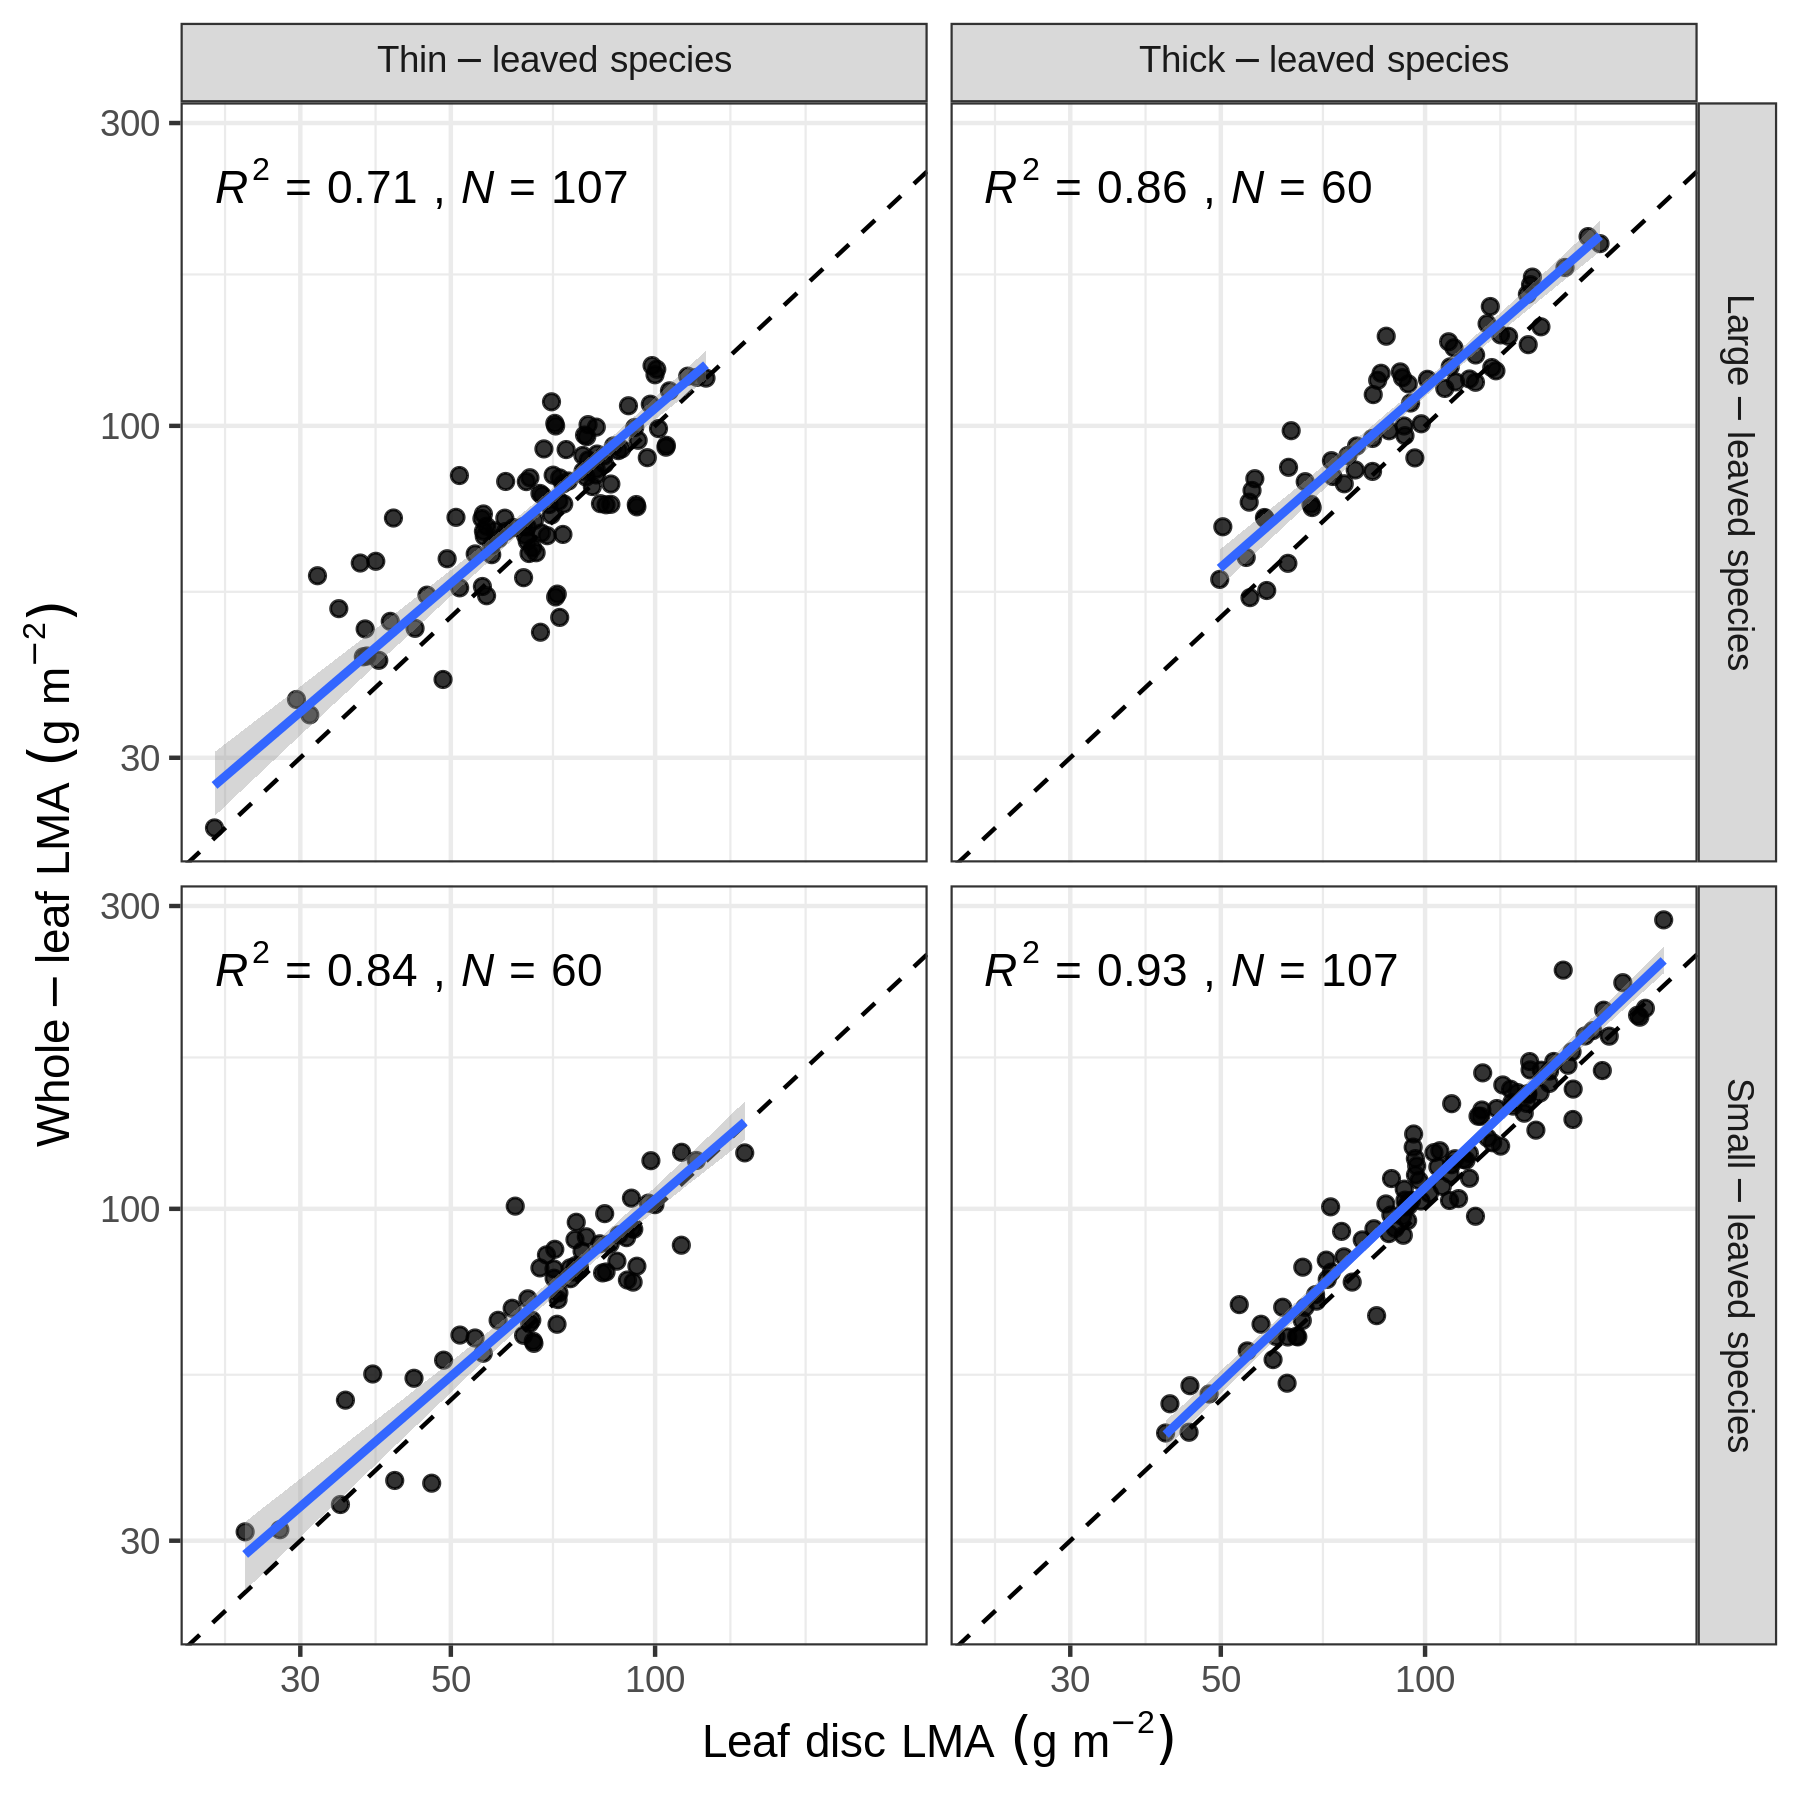
\includegraphics{../figs/lalt_pool_grid.png}
%DIFDELCMD < %%%
\DIFdelend \DIFaddbegin 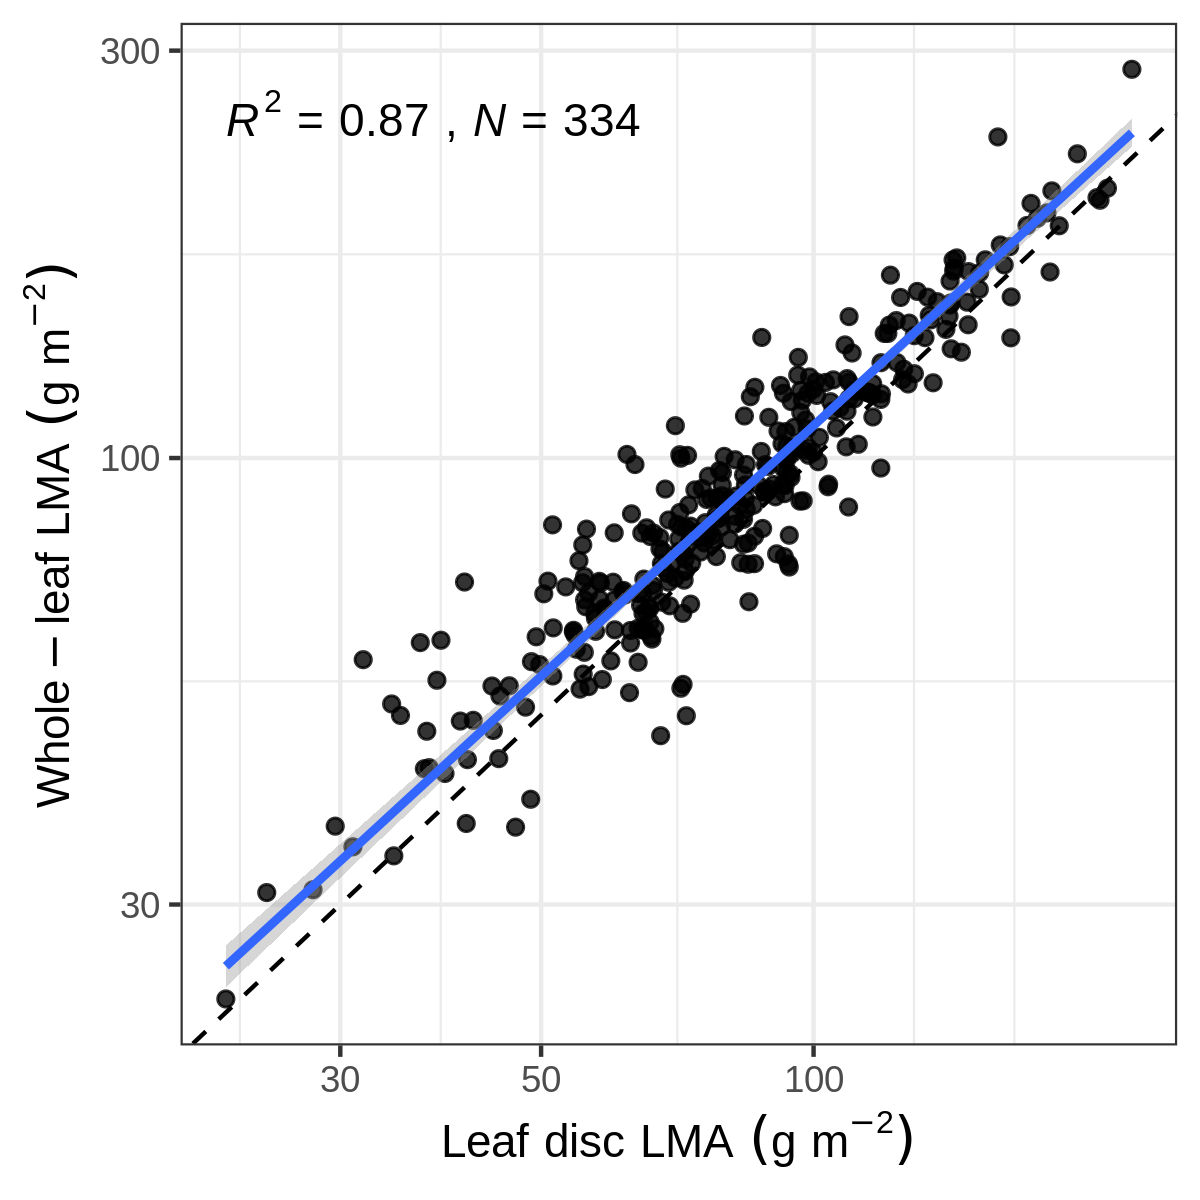
\includegraphics{../figs/sma.png}
\DIFaddend 

\newpage

\textbf{Fig. 2.}
\DIFdelbegin \DIFdel{Relationships between individual leaf mass per area
(LMA ) determined by using whole leaves and leaf discs.
Individual groups
are divided into four categories based on the basis of the medians of
the leaf size and leaf thickness across all the individuals}\DIFdelend \DIFaddbegin \DIFadd{Model predictions of the whole-leaf to leaf disc LMA ratio as a function of leaf punch sizes and (a) leaf tissue density, (b) leaf area, and (c) leaf thickness.
Dashed line indicates 1:1 ratio of leaf disc and whole-leaf estimates.
Solid lines indicate the posterior means (\(\tilde{\mu}\) in Eq. 1-2), and the shade regions shows \(\pm\) the posterior means of standard deviations (\(\tilde{\sigma}\) in Eq. 3-4).
}

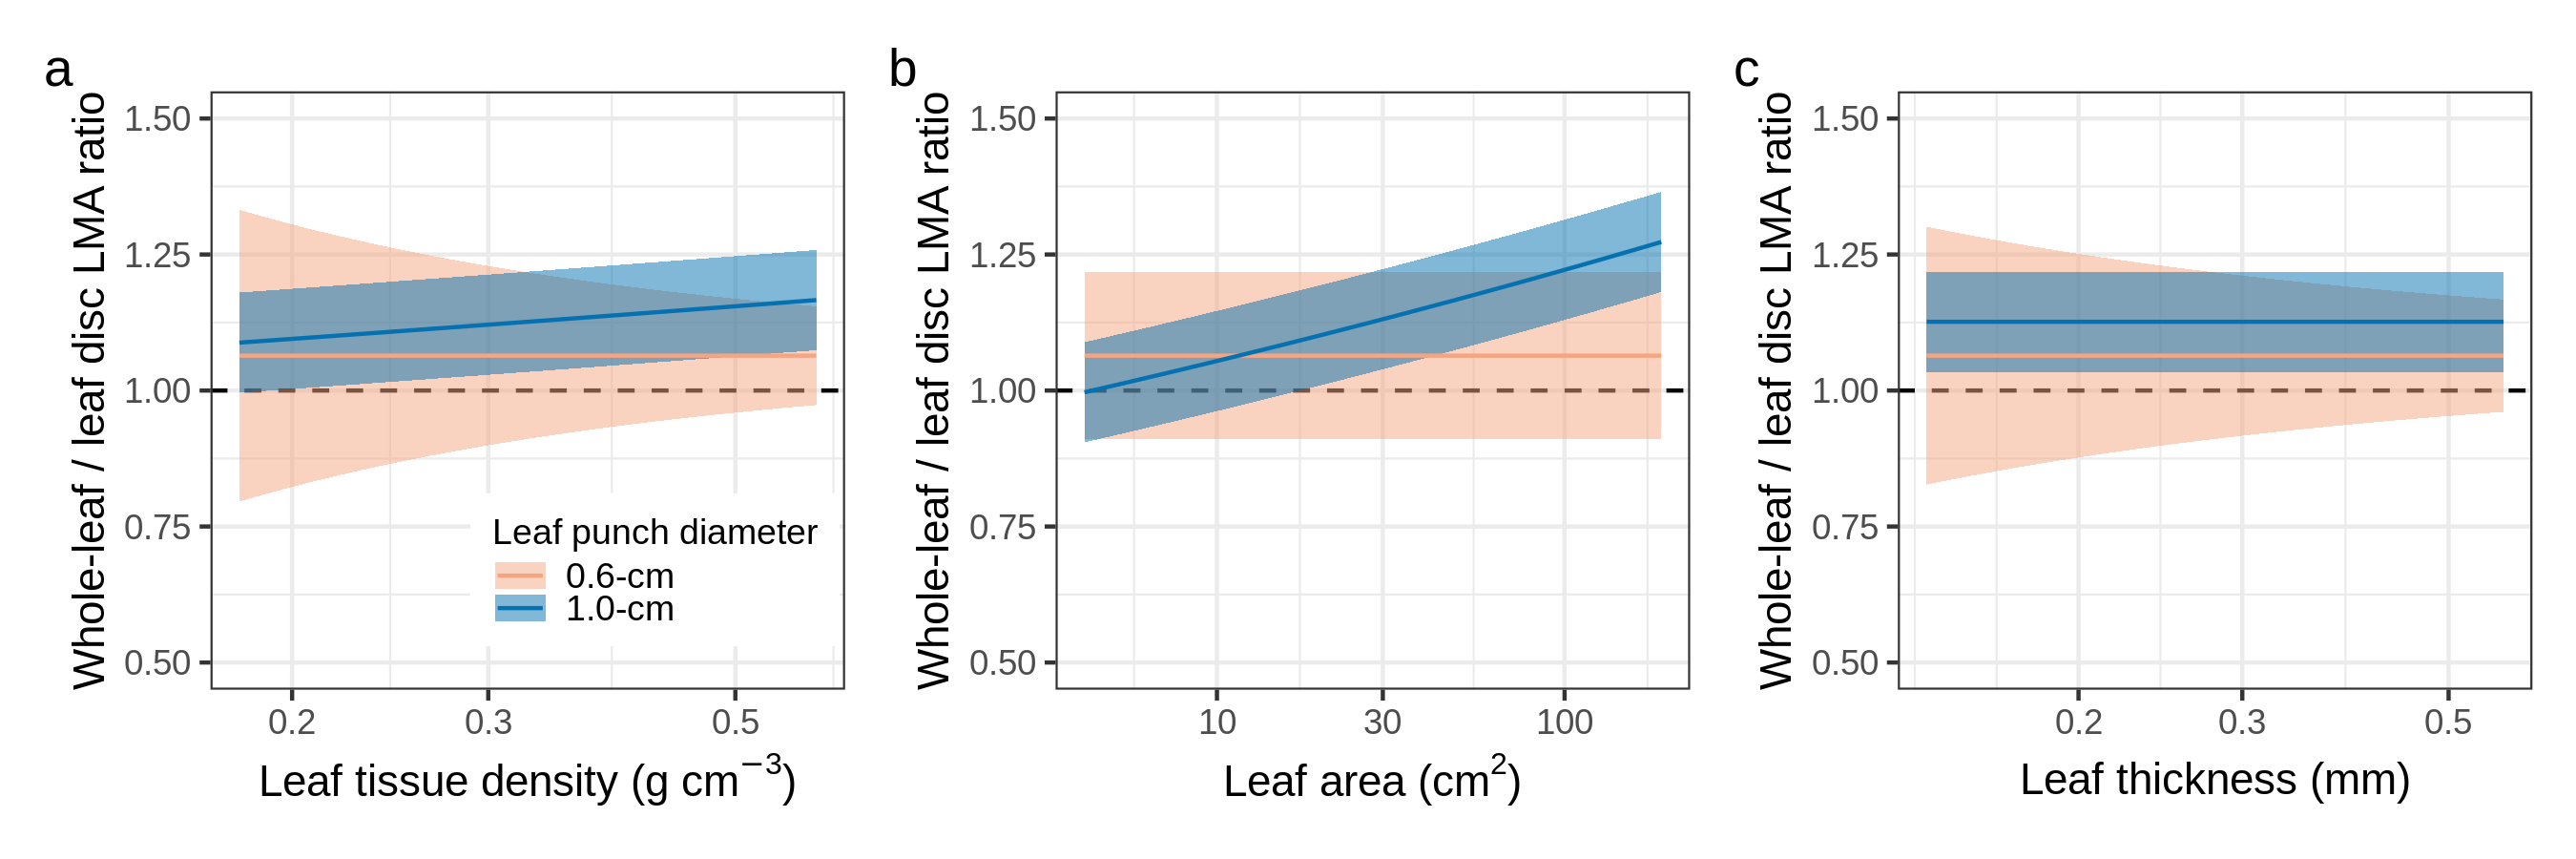
\includegraphics{../figs/pred_mcmc.png}

\newpage

\textbf{\DIFadd{Fig. 3.}}
\DIFadd{Relationships between petiole to leaf dry mass ratio and (a) leaf area and (b) whole-leaf to leaf disc LMA ratio.
Blue solid lines indicate ordinary least squares (OLS) regressions.
The 95\% confidence intervals are presented as the shaded area}\DIFaddend .
All the correlations are significant (\DIFdelbegin \emph{\DIFdel{P}} %DIFAUXCMD
\DIFdelend \DIFaddbegin \DIFadd{P }\DIFaddend \textless{} 0.001).
\DIFdelbegin \DIFdel{Details as in
Fig.
1.
}\DIFdelend \DIFaddbegin \DIFadd{All the samples were obtained with a diameter 1.0-cm leaf punch.
}\DIFaddend 

\DIFdelbegin %DIFDELCMD < 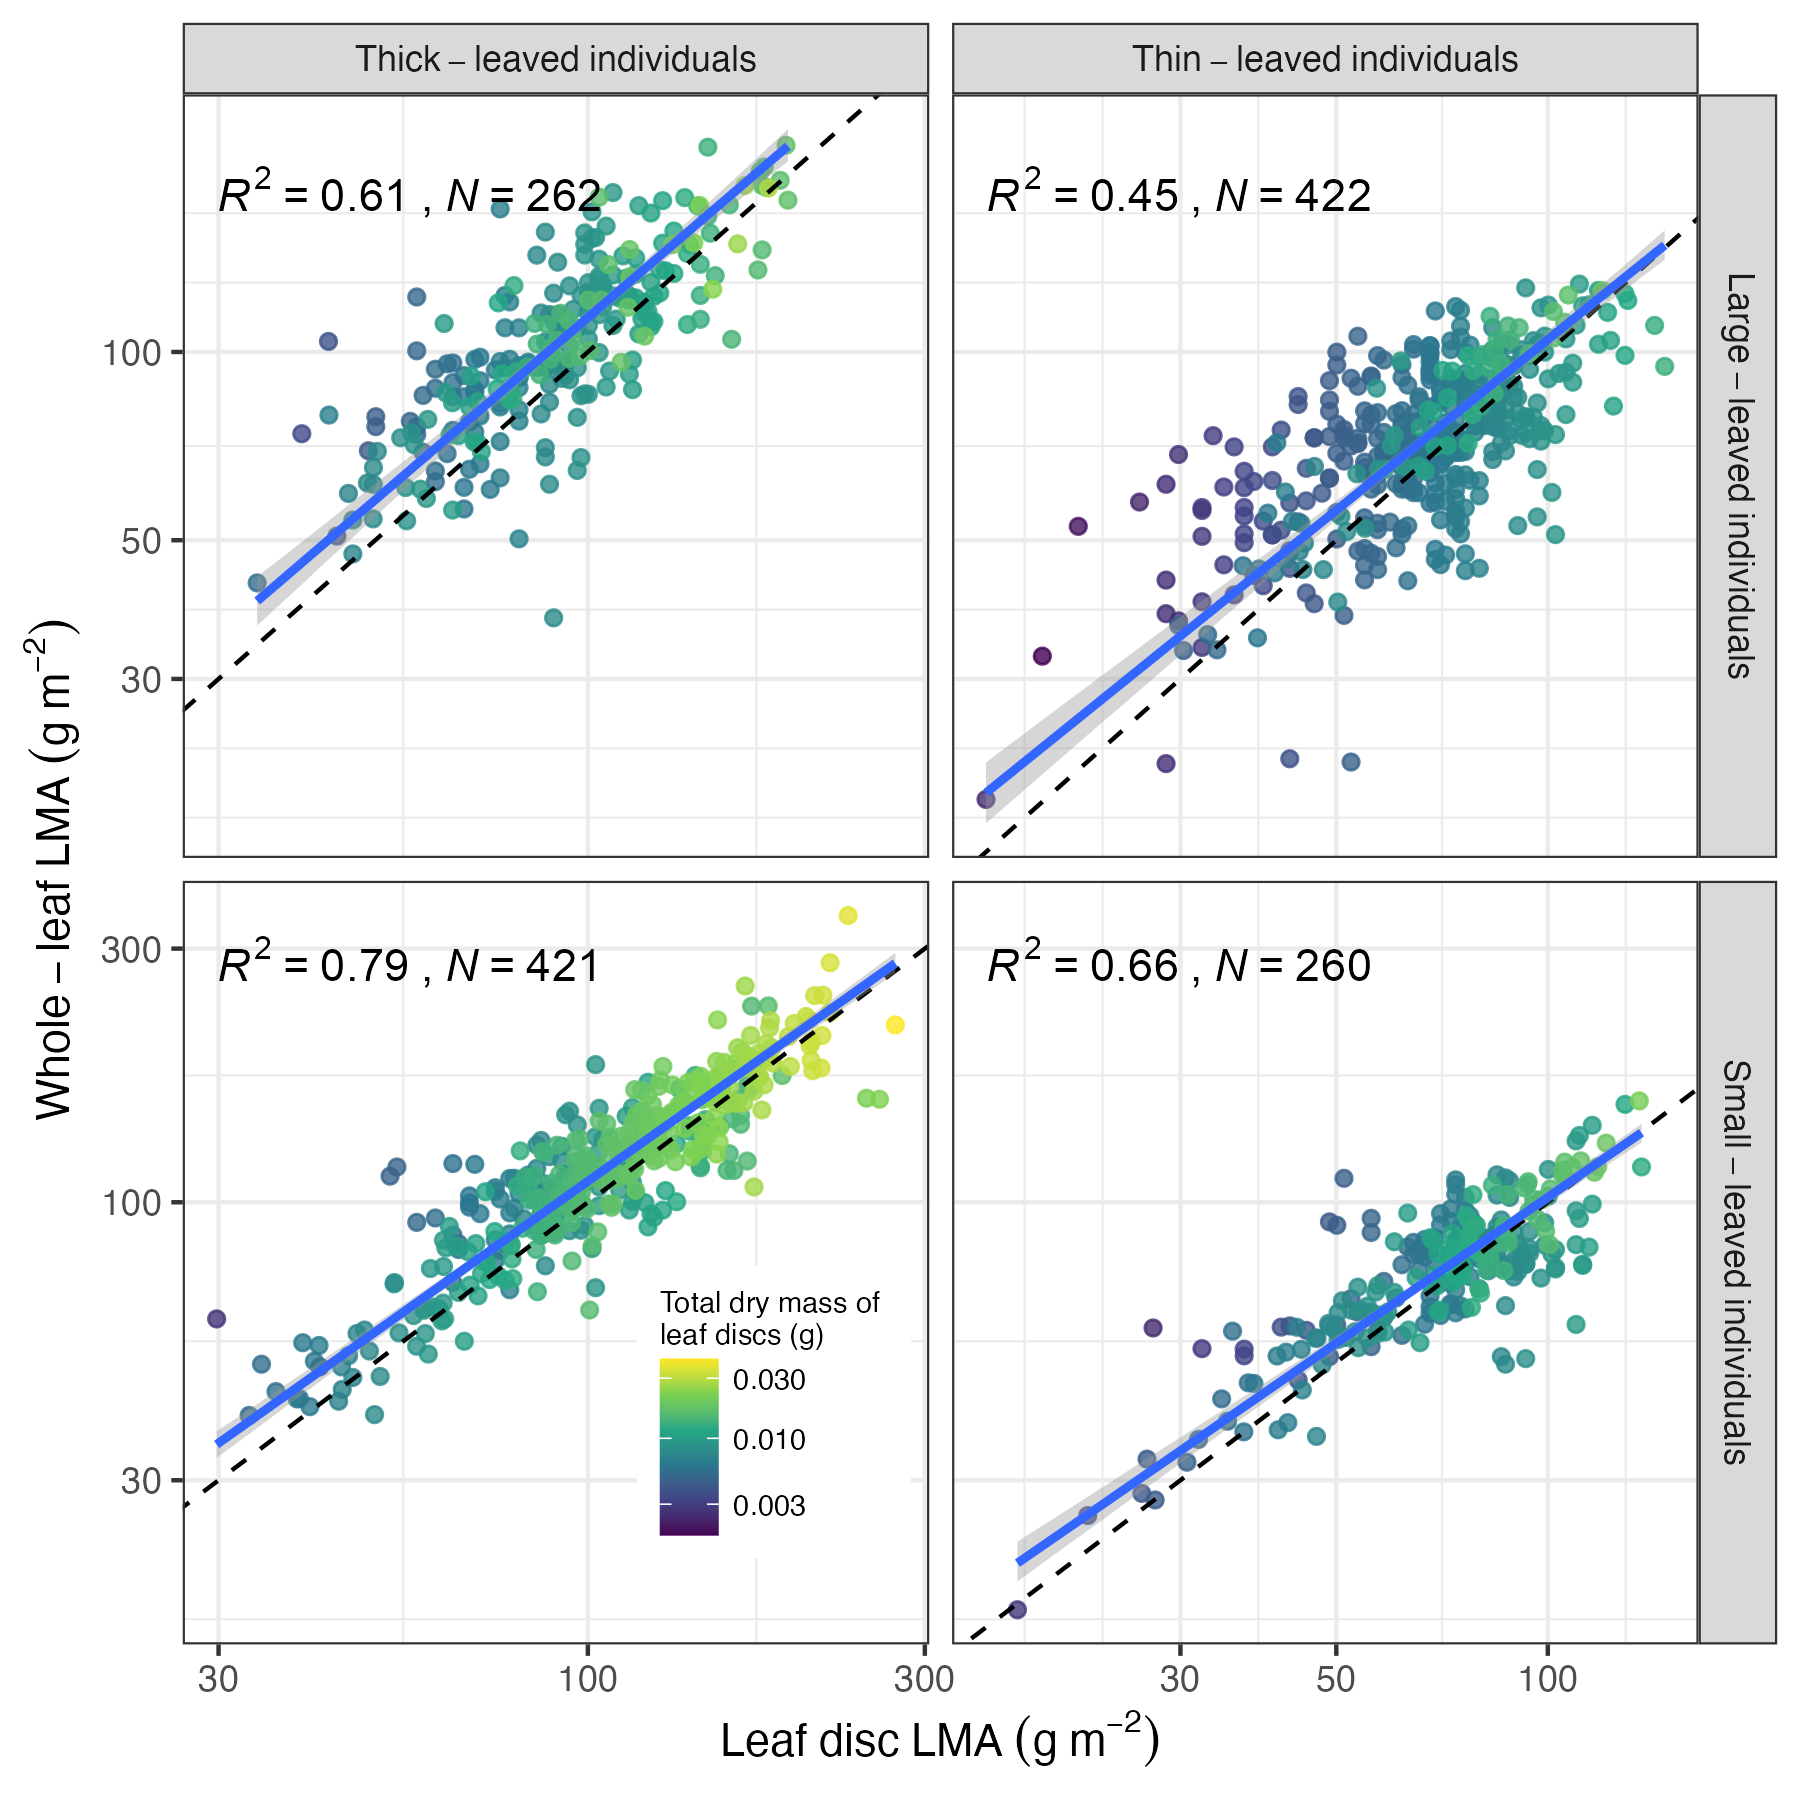
\includegraphics{../figs/lalt_tree_grid.png}
%DIFDELCMD < %%%
\DIFdelend \DIFaddbegin 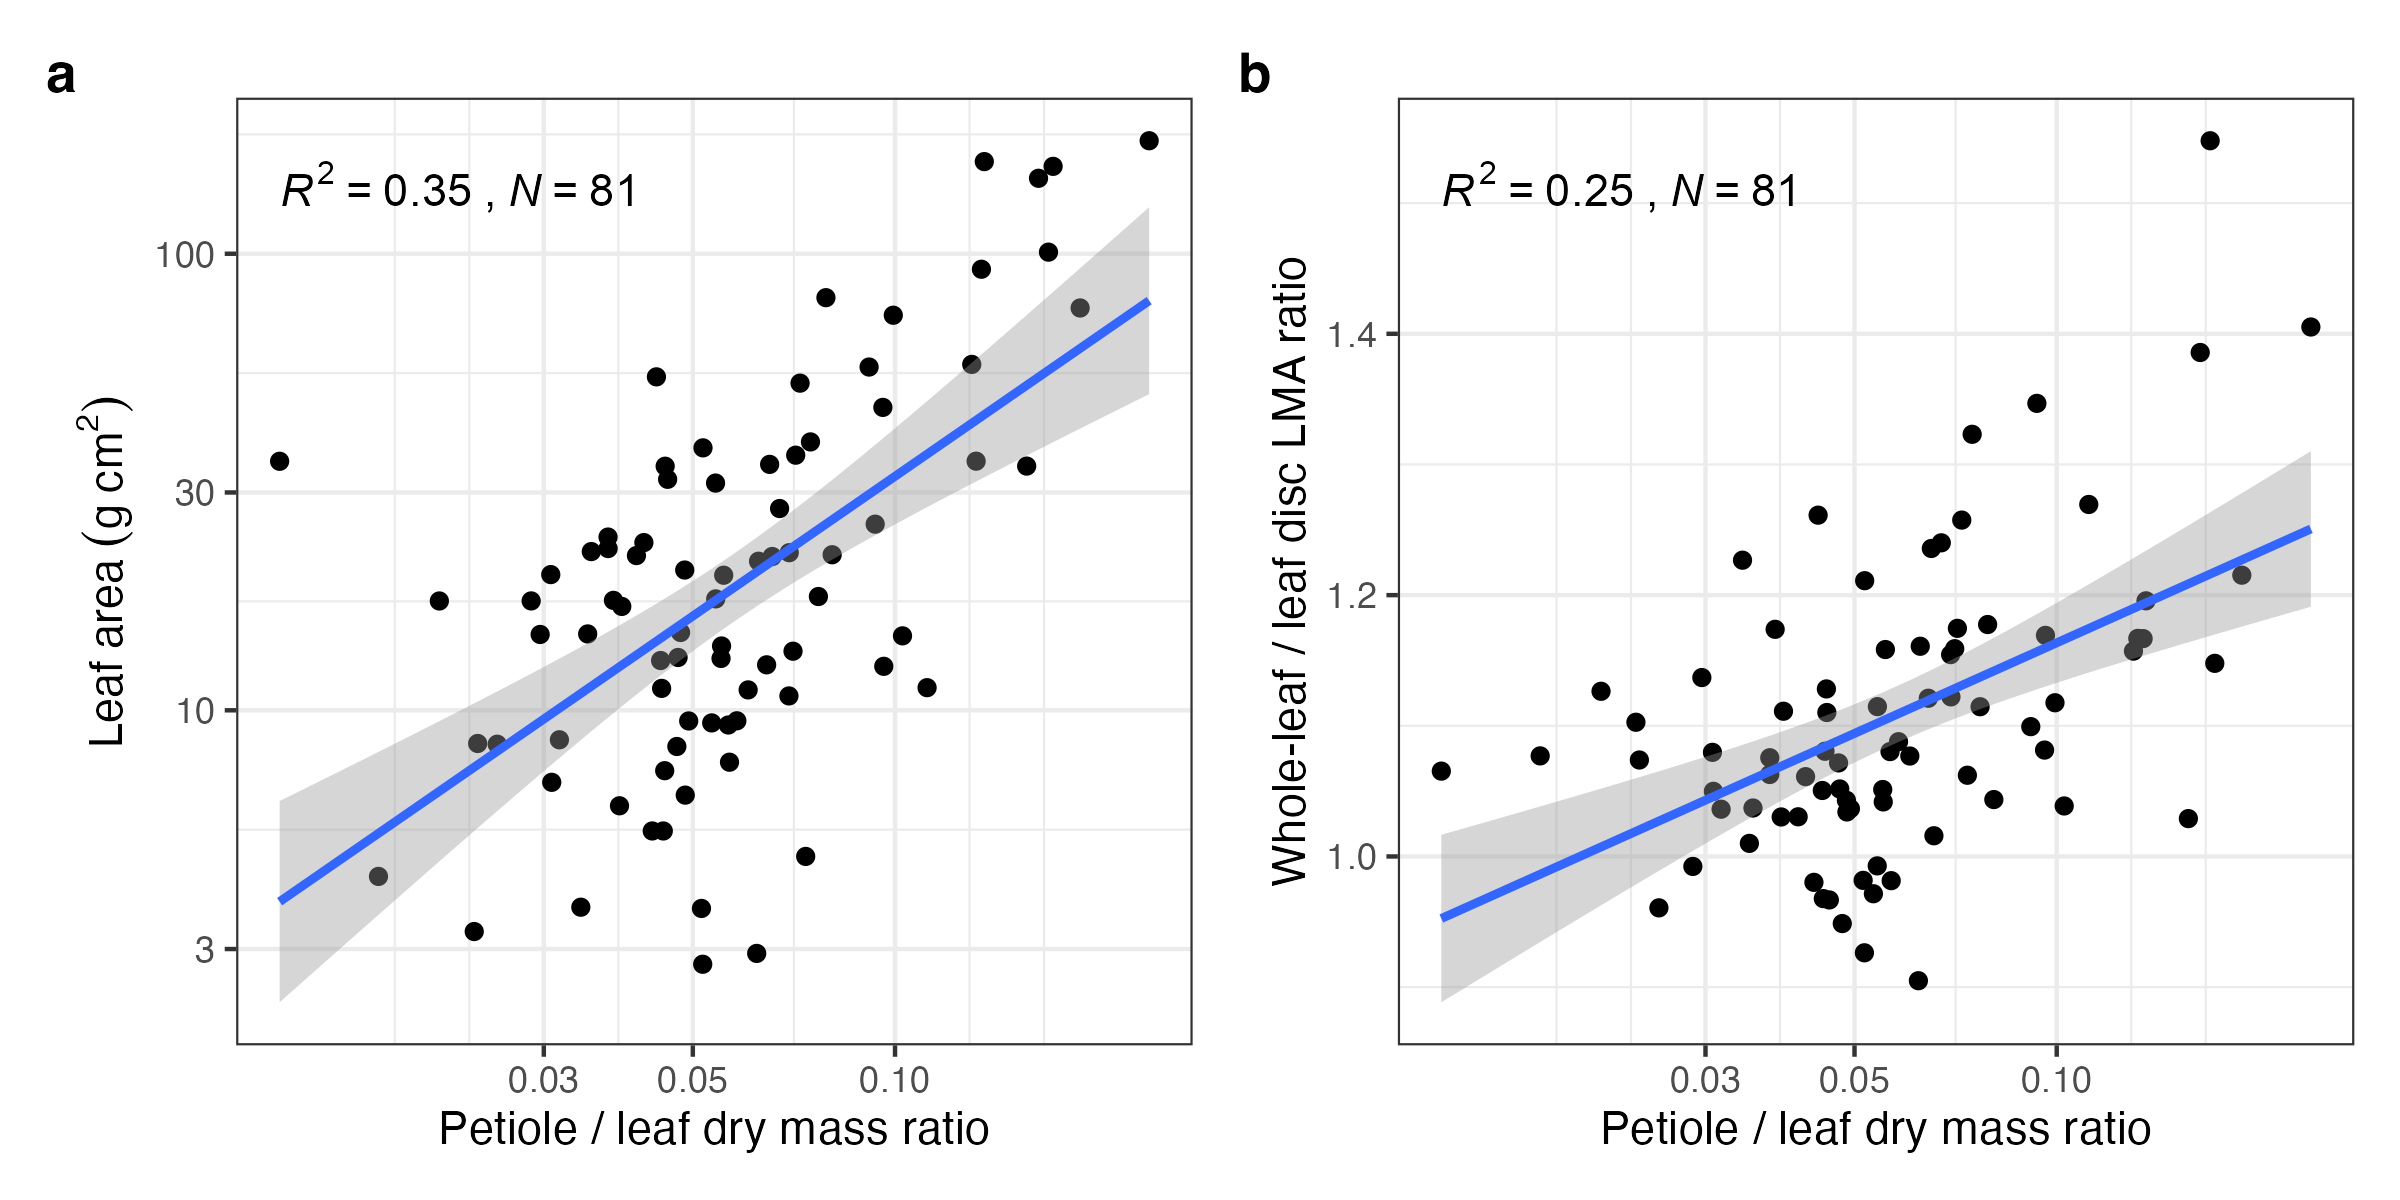
\includegraphics{../figs/petiole.png}
\DIFaddend 

\newpage

\textbf{Fig. \DIFdelbegin \DIFdel{3.}\DIFdelend \DIFaddbegin \DIFadd{4.}\DIFaddend }
Relationships between coefficient of variation (\DIFdelbegin \DIFdel{CV) in
leaf trait }\DIFdelend \DIFaddbegin \DIFadd{Bao's CV estimator, Eq. 5) in LMA }\DIFaddend values determined by using whole leaves and leaf discs\DIFdelbegin \DIFdel{: (a)
leaf mass per area (LMA)}\DIFdelend .
The correlation is significant (\emph{P} \textless{} 0.001).
Details as in Fig. 1.
\DIFdelbegin \DIFdel{Note that the axes are square
root scales.
}\DIFdelend 

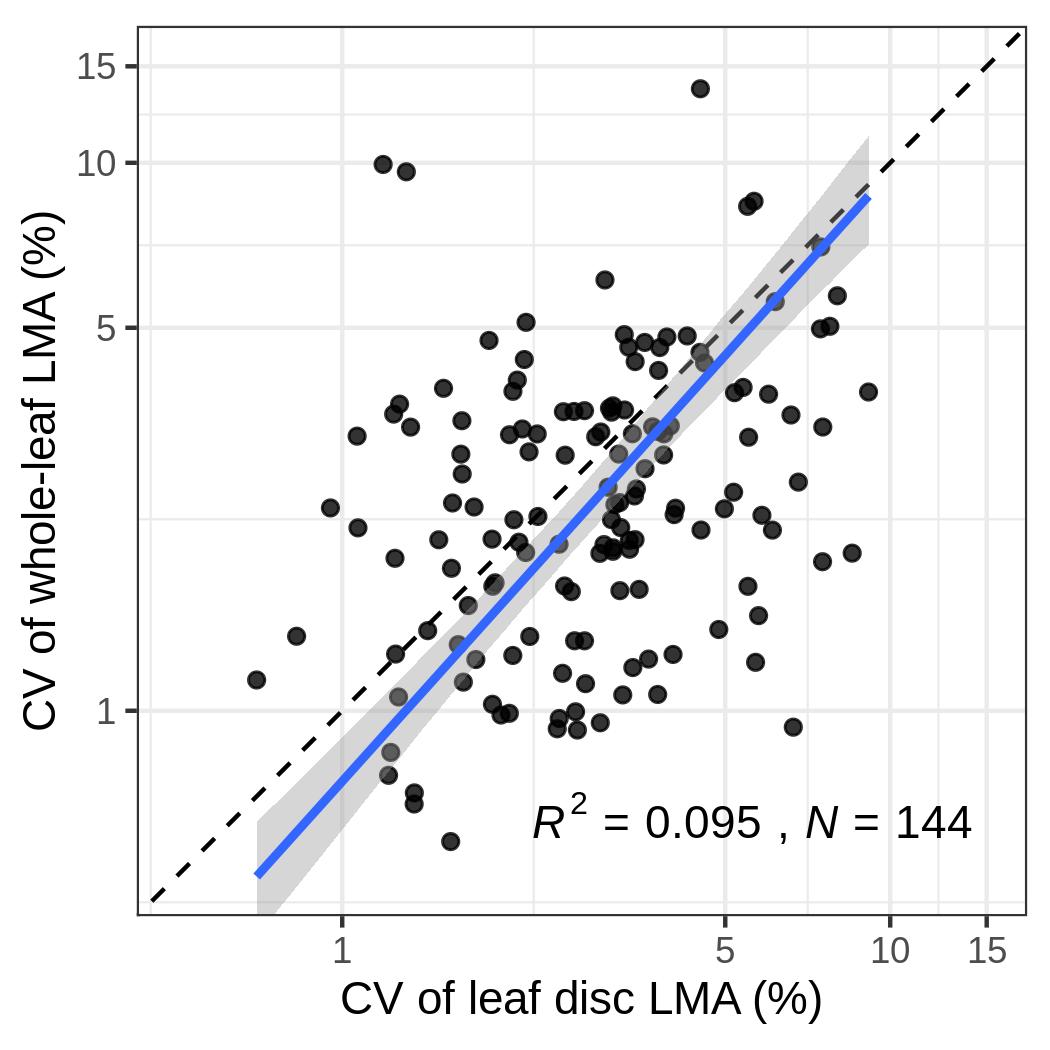
\includegraphics{../figs/cv_pool.png}

\end{document}
